\documentclass[aps,prb,10pt,twocolumn,superscriptaddress,longbibliography,floatfix]{revtex4-2}
\usepackage{amsmath,amssymb,amsthm}
\usepackage{float}
\usepackage{placeins}   % keep floats within their major manuscript sections
\usepackage{needspace}
\usepackage{graphicx}
\usepackage{capt-of}
\graphicspath{{figures/}}
\usepackage[colorlinks=true,urlcolor=blue,linkcolor=blue,citecolor=blue]{hyperref}
\usepackage[dvipsnames]{xcolor}
\pdfstringdefDisableCommands{\def\newtext#1{#1}}
\usepackage{bm}
\usepackage{soul}
\usepackage{pifont}
\usepackage{mathtools}
\usepackage{tikz}
\usetikzlibrary{tikzmark,arrows.meta,positioning,shapes.geometric,calc}
\usepackage{array}
\usepackage[normalem]{ulem}
\usepackage{mdframed}
\usepackage{enumitem}
\usepackage{makecell}
\usepackage{physics}
\usepackage{comment}

\DeclareMathOperator\arctanh{arctanh}
\DeclareMathOperator{\Sgn}{Sgn}

% ── Shorthands ──
\newcommand{\ii}{\mathrm{i}}
\newcommand{\mc}[1]{\mathcal{#1}}
\newcommand{\mr}[1]{\mathrm{#1}}
\newcommand{\mf}[1]{\mathfrak{#1}}
\newcommand{\mb}[1]{\mathbb{#1}}
\newcommand{\mbf}[1]{\mathbf{#1}}
\newcommand{\bs}[1]{\boldsymbol{#1}}
\newcommand{\h}[1]{\hat{#1}}
\newcommand{\Id}{\mathbf{1}}

% ── Physics objects ──
\newcommand{\bfr}{\boldsymbol r}
\newcommand{\bk}{\boldsymbol k}
\newcommand{\kett}[1]{\ket{#1}\!\rangle}
\newcommand{\braa}[1]{\langle\!\bra{#1}}
\newcommand{\CI}{\kett{\mr{CI}}}
\newcommand{\fSWAP}{\operatorname{fSWAP}}
\newcommand{\rec}{\mathbf m}   % measurement record

% ── Draft annotation ──
\newcommand{\drafthighlight}[1]{\textcolor{red}{#1}}
\newcommand{\cmjadd}[1]{\drafthighlight{#1}}
\newcommand{\abadd}[1]{\drafthighlight{#1}}
\newcommand{\HPadd}[1]{\drafthighlight{#1}}
\newcommand{\cmjCom}[1]{\textcolor{red}{[CMJ: #1]}}
\newcommand{\abcom}[1]{\textcolor{purple}{[AB: #1]}}
\newcommand{\HPcom}[1]{\textcolor{cyan}{[HP: #1]}}
\newcommand{\newtext}[1]{{\color{blue}#1}}
\newcommand{\GPT}[1]{{\color{magenta}[GPT: #1]}}
\newcommand{\claudeadd}[1]{{\color{orange}#1}}
\newcommand{\claudecom}[1]{{\color{ForestGreen}[Claude: #1]}}
\newcommand{\claudedel}[1]{{\color{orange}\sout{#1}}}

% RevTeX 4.2f: check a deferred float only after an eligible-width pass.
% This preserves layout and genuine stuck-float detection in the column pass.
\makeatletter
% Delay the unchanged-queue check when the full-width pass has no eligible float.
% The ordinary column pass still diagnoses a truly unplaceable column float.
\let\manuscript@check@deferlist@stuck\check@deferlist@stuck
\def\check@deferlist@stuck#1{%
  \ifx#1\do@startpage
    \begingroup
    \def\manuscript@next{\endgroup}%
    \def\@elt##1{%
      \ifdim\wd##1<\textwidth\else
        \def\manuscript@next{\endgroup\manuscript@check@deferlist@stuck#1}%
      \fi}%
    \@deferlist
    \manuscript@next
  \else
    \manuscript@check@deferlist@stuck#1%
  \fi}
\makeatother


\begin{document}
\raggedbottom

\title{Chiral Domain Wall Modes in Adaptive Quantum Dynamics}
\author{Asadullah Bhuiyan, Haining Pan, Chao-Ming Jian}
\noaffiliation
\date{\today}

\begin{abstract}
\newtext{We demonstrate a two-dimensional adaptive free-fermion circuit for preparing chiral critical boundary states using finite-range occupation measurements and local feedback, without postselection. Fresh ancillary modes correct every undesired outcome, giving an equivalent description in terms of monitored fermion gain and loss. Spatially varying the protocol creates interfaces between a Chern slab and a trivial exterior. Numerical results show bulk Chern preparation together with algebraic correlations and logarithmic entanglement and charge fluctuations along the interfaces in the conditioned pure states. Wall-resolved entropy and opposite modular propagation on the two interfaces are consistent with one chiral complex-fermion branch per wall. These signatures characterize the boundary states without requiring an identification with a particular equilibrium ground state. The same interfaces host slow purification modes, whose spatial profiles and finite-time Lyapunov gaps connect the prepared boundary physics to the dynamics. Discarding the measurement record leaves short-range two-point correlations and a finite relaxation gap in the outcome-averaged channel; we relate this gap to its single-particle representation. The critical boundary signatures thus reside in the conditioned trajectories and are lost upon outcome averaging.}
\end{abstract}

\maketitle

\setcounter{tocdepth}{2}
\tableofcontents

\section{Introduction}

Dynamical quantum systems involving both unitary evolution and stochastic wavefunction collapse from measurements provide a rich setting for new types of non-equilibrium matter~\cite{PotterVasseur2022,FisherKhemaniNahumVijay2023}.
In particular, the discovery of measurement-induced phase
transitions~\cite{LiChenFisher2018,SkinnerRuhmanNahum2019,ChanNandkishorePretkoSmith2019,LiChenFisher2019,GullansHuse2020}
sparked rapid progress in our understanding of non-equilibrium physics. The landscape of such transitions is further enriched by global symmetries~\cite{SangHsieh2021,BaoChoiAltman2021,LavasaniAlaviradBarkeshli2021,AgrawalEtAl2022,BarrattEtAl2022,MajidyEtAl2023}, reshaped by unitary feedback conditioned on measurement outcomes~\cite{IadecolaEtAl2023,RavindranathEtAl2023,PiroliEtAl2023,SierantTurkeshi2023,ODeaEtAl2024}, and qualitatively modified by
decoherence~\cite{WeinsteinBaoAltman2022,LiSangHsieh2023,LiuLiZhangJian2024,IvakiOjanenMoghaddam2025}.

In this work, we seek to better understand the role of topology in these dynamical systems. In equilibrium, topological phases, such as Chern insulators, are a staple in
the study of quantum matter. For free fermion systems, topological phases are \claudedel{organized according to symmetry and dimensionality tenfold way}\claudeadd{organized by symmetry and dimensionality into the tenfold way}~\cite{AltlandZirnbauer1997,SchnyderRyuFurusakiLudwig2008,Kitaev2009,RyuSchnyderFurusakiLudwig2010,ChiuTeoSchnyderRyu2016}.
Such phases cannot be smoothly deformed into a topologically distinct phase without closing the gap or breaking the relevant symmetry. At the interface between distinct bulk topological phases, boundary-localized, gapless modes robust against symmetry-preserving
perturbations emerge~\cite{Halperin1982,Hatsugai1993,TeoKane2010}. This bulk-boundary correspondence is a cornerstone of both experimental and theoretical condensed matter physics~\cite{HasanKane2010,QiZhang2011}. A key feature of these phases is their robustness to spatial disorder. In particular, the bulk invariant survives gap-preserving spatial disorder, such that chiral boundary modes 
evade Anderson localization~\cite{Halperin1982,EversMirlin2008}. Monitored dynamics provides a new arena in which to study this robustness, since the randomness of measurement outcomes acts as spatiotemporal disorder~\cite{JianBauerKeselmanLudwig2022}. \claudedel{Distinct from typical disorder however, Born rule are subject to temporal disorder that is correlated with the state itself}\claudeadd{Unlike typical disorder, however, Born-rule outcomes constitute temporal disorder that is correlated with the state itself}~\cite{JianShapourianBauerLudwig2023,FavaEtAl2023}. \claudeadd{This matters for gapless boundaries in particular: nonchiral free fermions in one dimension generically lose their critical correlations under random measurements at long scales~\cite{PoboikoEtAl2023}, so it is not a priori clear that measurement-induced randomness spares a chiral boundary.}

Recently, the role of topology in monitored quantum dynamics has advanced notably, particularly for free fermions. Concrete $1+1$D models with topologically distinct area-law phases have been identified~\cite{KellsMeidanRomito2023,BehrendsVennBeri2024,PanShapourianJian2025,Oshima2025, yang2026decoding}, while Refs.~\cite{BhuiyanPanJian2026,XiaoKawabata2026} develop topological classifications of free-fermion monitored dynamics based on the AZ symmetry classification.

There has also been notable progress in the physics of boundary modes in topological dynamical phases.  Refs.~\cite{PanShapourianJian2025, Oshima2025} identified dynamical topological modes localized on $0+1$D domain walls between $1+1$D topological dynamical phases. Ref.~\cite{XiaoKawabata2026}
established an analog of the bulk-boundary correspondence in which non-trivial bulk topology corresponds to the gapless modes in the Lyapunov spectrum of the dynamics. Their $2+1$D construction, however, postselects the measurement outcomes, so it is unclear whether chiral boundary modes survive genuine stochastic, monitored dynamics. Whether chiral, gapless boundary modes can be realized under genuine Born-rule dynamics is of interest to this work.

\claudeadd{The question is also natural from the perspective of state preparation. A single chiral branch is anomalous: it can only exist at the boundary of a two-dimensional region with nonzero Chern number. Preparing it therefore requires preparing a chiral bulk, which strictly local finite-depth unitary circuits cannot do~\cite{LuLessaKimHsieh2022}, and which finite-range dissipative dynamics cannot stabilize as a pure steady state~\cite{BardynEtAl2013,BudichZollerDiehl2015,Goldstein2019}. Adaptive circuits that combine measurements with classical feedforward circumvent some of these constraints. Reference~\cite{LuLessaKimHsieh2022} prepares chiral topological order in constant depth, given a chiral free-fermion resource state, and one-dimensional critical states in logarithmic depth using nonlocal classical communication. Here we ask whether a much simpler ingredient, repeated finite-range measurements with purely local feedback, can prepare chiral critical boundaries directly. We find that it can, but at the level of individual trajectories: each measurement record yields a pure state whose walls are critical and chiral, whereas the outcome-averaged state is short-range correlated.}
\claudecom{This paragraph is meant to replace the GPT novelty note below, which can then be deleted. Double-check that the summary of Ref.~\cite{LuLessaKimHsieh2022} matches your reading: they explicitly state that strictly local finite-depth unitaries cannot prepare a $p+\ii p$ state, and they obtain it by adiabatic evolution.}

In this paper, we consider a 2+1D adaptive quantum circuit consisting of finite-range occupation measurements, local unitary feedback, and ancilla modes. The adaptive circuit steers towards the topological phase by measuring truncated, overcomplete Wannier (OW) modes and swapping in fresh ancilla modes with the target occupancy whenever an undesired occupancy is observed. \claudedel{For finite-range OW measurements, the overcompleteness leads to measurement-outcome frustration and so does not steer towards a common dark state.}\claudeadd{For finite-range OW measurements, truncation mixes the two bands, so the stabilizers are frustrated and no common dark state exists. This frustration is unavoidable: compactly supported single-particle functions cannot both lie within a Chern band and span it at every momentum~\cite{DubailRead2015}.} Instead, the dynamics approach a disordered ensemble of Chern insulator states.
\GPT{The frustration is caused by finite-range truncation and band mixing, rather than overcompleteness alone: the untruncated OW stabilizers share a common dark state.}
 
By tracing out ancilla degrees of freedom, we show that unitary feedback becomes equivalent to fermion-counting operations on the physical system, consisting of particle gain and loss operations in the OW basis that correct undesired measurement outcomes. This simplified model will be the main system of interest in this work.

{\color{blue}
We then introduce programmable domain walls by making the circuit parameter $\alpha$ spatially dependent. We first verify that the circuit prepares a topological bulk within the slab, and then show that purification remains slow at its boundaries. The pure states prepared along individual trajectories have algebraic wall correlations and logarithmic entanglement and charge fluctuations. Their restricted spectra provide a complementary view: the number of partially occupied modes grows with the logarithm of the subsystem chord length. We examine the convergence of the entropy coefficient, resolve its contribution from each wall, and use modular evolution to identify opposite chiralities. Together, these results provide evidence for critical chiral boundary states under finite-range, postselection-free adaptive dynamics\claudedel{; they do not establish that the circuit prepares an equilibrium chiral-Luttinger-liquid ground state}\claudeadd{. We do not claim that the conditioned wall states coincide with the ground state of an equilibrium chiral Luttinger liquid; our evidence concerns their universal correlations, entanglement, and handedness.} Finally, we discard the measurement record and find short-range two-point correlations and a finite relaxation gap for the averaged channel over the sizes studied. The boundary criticality diagnosed here thus resides in the conditioned trajectories.
}



\GPT{For the novelty claim, compare with Ref.~\cite{LuLessaKimHsieh2022}, which gives adaptive constructions of chiral topological order and, separately, critical states. The distinction here is the repeated finite-range measurement-and-local-feedback preparation of critical chiral boundaries under Born sampling.}

\section{Topological Adaptive Circuit with Domain Walls}
\label{sec:Model}

In this section, we construct the adaptive circuit studied in the rest of this work. It is a variant of the topological adaptive circuit of Ref.~\cite{BhuiyanPanJian2026}, which steers a two-dimensional fermionic system toward a Chern insulator by repeatedly measuring localized stabilizers and correcting undesired outcomes with unitary feedforward operations. We make two modifications. First, we replace the finite ancillary bath of Ref.~\cite{BhuiyanPanJian2026} by a supply of fresh ancillas, so that every undesired outcome is corrected. Once the ancillas are traced out, the feedforward operations reduce to single-fermion gain and loss, i.e., to fermion counting. Second, we let the parameter \claudedel{which}\claudeadd{that} controls the steady-state topological phase vary in space, which introduces domain walls between topologically distinct dynamical phases.

In Sec.~\ref{sec:Stabilizers}, we review the stabilizer formalism introduced in Ref.~\cite{BhuiyanPanJian2026} for a Chern insulator in terms of overcomplete Wannier (OW) modes, truncate the OW modes to a finite range, and introduce the domain walls. In Sec.~\ref{sec:Circuit}, we present the measurement-and-feedforward operation with fresh ancillas, assemble these ingredients into the adaptive circuit, and describe its numerical implementation.



\subsection{Stabilizers, truncation, and domain walls}
\label{sec:Stabilizers}

We target a Chern insulator $\CI$ given by the half-filled ground state of a variant of the Qi--Wu--Zhang (QWZ) Hamiltonian~\cite{QiWuZhang2006}. The system is defined on a 2d square lattice with two fermion modes $\hat c_{\bfr,1}$ and $\hat c_{\bfr,2}$ per unit cell, where the unit-cell coordinate $\bfr=(x,y)\in\mathbb Z^2$ is a pair of integers. With the Fourier convention $\hat c_\mu(\bk)=\sum_{\bfr}e^{\ii\bk\cdot\bfr}\hat c_{\bfr,\mu}$, the parent Hamiltonian reads
\begin{align}
    \hat H_{\mr{CI}}&=\int_{\mr{BZ}}\frac{d^2\bk}{(2\pi)^2}\,
    \hat c^\dagger(\bk)\big[\boldsymbol n(\bk)\cdot\boldsymbol\sigma\big]\hat c(\bk),\nonumber\\
    \boldsymbol n(\bk)&=(\sin k_x,\ \sin k_y,\ \alpha-\cos k_x-\cos k_y).
    \label{eq:QWZ}
\end{align}
Here, $\boldsymbol\sigma$ is the vector of Pauli matrices, $\hat c(\bk)=(\hat c_1(\bk),\hat c_2(\bk))^{\mathsf T}$, and $\alpha\in\mathbb R$ tunes the target state. The Chern insulator $\CI$ fully occupies the lower band of $\hat H_{\mr{CI}}$ and leaves the upper band empty.  Here and below, the double ket $\kett{\cdots}$ denotes many-body states and the single ket $|\cdots\rangle$ single-particle states. The band gap is finite for $\alpha\neq0,\pm2$, which we assume unless stated otherwise. The single-particle projectors onto the upper ($\sigma=+$) and lower ($\sigma=-$) bands are $P_\sigma(\bk)=\frac12[\Id+\sigma\,\hat{\boldsymbol n}(\bk)\cdot\boldsymbol\sigma]$, with $\hat{\boldsymbol n}=\boldsymbol n/|\boldsymbol n|$.
We define the Chern number of $\CI$ as that of its occupied band,
\begin{equation}
    \mc C=\frac{1}{2\pi\ii}\int_{\mr{BZ}}d^2\bk\,
    \operatorname{tr}\!\Big(P_-\big[\partial_{k_x}P_-,\partial_{k_y}P_-\big]\Big),
    \label{eq:ChernNumber}
\end{equation}
which gives $\mc C=1$ for $\alpha\in(0,2)$, $\mc C=-1$ for $\alpha\in(-2,0)$, and $\mc C=0$ for $|\alpha|>2$. Note that our convention is related to that of Ref.~\cite{BhuiyanPanJian2026} by $\alpha\to-\alpha$.

Following Ref.~\cite{BhuiyanPanJian2026}, we describe $\CI$ using localized stabilizers built from OW modes. Concretely, we project a local trial orbital onto either band,
\begin{equation}
    W_{\bfr,\nu,\sigma}(\bfr',\mu)\propto\int_{\mr{BZ}}\frac{d^2\bk}{(2\pi)^2}\,
    e^{\ii\bk\cdot(\bfr-\bfr')}\big[P_\sigma(\bk)\,\tau_\nu\big]_\mu,
    \label{eq:OWWavefunction}
\end{equation}
where $[\cdots]_\mu$ denotes the $\mu$th component and the proportionality constant normalizes $W_{\bfr,\nu,\sigma}$. We use the two eigenvectors of $\sigma^x$ as trial orbitals, $\tau_A=(1,1)^{\mathsf T}/\sqrt2$ and $\tau_B=(1,-1)^{\mathsf T}/\sqrt2$. The associated OW fermion operators and their number operators are $\hat\chi^\dagger_{\bfr,\nu,\sigma}=\sum_{\bfr',\mu}W_{\bfr,\nu,\sigma}(\bfr',\mu)\,\hat c^\dagger_{\bfr',\mu}$ and $\hat{\mc N}_{\bfr,\nu,\sigma}=\hat\chi^\dagger_{\bfr,\nu,\sigma}\hat\chi_{\bfr,\nu,\sigma}$.
Since $W_{\bfr,\nu,\sigma}$ is normalized, each $\hat{\mc N}_{\bfr,\nu,\sigma}$ is a projector with eigenvalues 0 and 1. For $\alpha\neq0,\pm2$, $W_{\bfr,\nu,\sigma}$ is exponentially localized around $\bfr$, with a localization length that diverges as the band gap closes. The parameter $\alpha$ thus controls both the topology of the target state and the range of the OW modes.

For a band with nonzero Chern number, a single family of OW modes cannot span the band. Writing $P_\sigma(\bk)=|u_\sigma(\bk)\rangle\langle u_\sigma(\bk)|$, the weight of the family $\nu$ at momentum $\bk$ is set by the overlap $\langle u_\sigma(\bk)|\tau_\nu\rangle$, which must vanish somewhere in the Brillouin zone~\cite{LiDongLedwithKhalaf2024,BhuiyanPanJian2026}. The two families together, however, do span the band, since $\tau_A$ and $\tau_B$ form an orthonormal basis and hence $\sum_{\nu}|\langle u_\sigma(\bk)|\tau_\nu\rangle|^2=1$ for every $\bk$. This overcompleteness guarantees that $\CI$ is the unique many-body state satisfying the stabilizing conditions $\hat{\mc N}_{\bfr,\nu,-}\CI=\CI$ and $(\hat\Id-\hat{\mc N}_{\bfr,\nu,+})\CI=\CI$ for all $\bfr$ and $\nu=A,B$. The first condition fills every lower-band OW mode and hence the entire lower band, while the second empties the entire upper band.

Note that these stabilizers do not always commute. For two OW modes $a$ and $b$ of the same band, $[\hat{\mc N}_a,\hat{\mc N}_b]=\langle W_a|W_b\rangle\,\hat\chi^\dagger_a\hat\chi_b-\mr{h.c.}$, which is nonzero whenever the two modes overlap. Nevertheless, the stabilizing conditions are frustration free: $\CI$ satisfies all of them simultaneously.

\label{sec:TruncatedOW}
While exponentially localized, the OW modes are supported on the entire lattice. To obtain a circuit with strictly finite-range operations, we truncate each OW function to a $(2w+1)\times(2w+1)$ window around its center and renormalize it,
\begin{equation}
    \widetilde W_{\bfr,\nu,\sigma}(\bfr',\mu)\propto g_{w,\bfr}(\bfr')\,W_{\bfr,\nu,\sigma}(\bfr',\mu),
    \label{eq:TruncatedOW}
\end{equation}
where $g_{w,\bfr}(\bfr')=1$ if $|x-x'|\leq w$ and $|y-y'|\leq w$ (distances on the periodic lattice) and $g_{w,\bfr}(\bfr')=0$ otherwise. In the figures, the truncation range $w$ is denoted by $n_{\rm shell}$. Throughout the main text, we use $w=1$, i.e., $3\times3$ windows. Henceforth, $\hat\chi_{\bfr,\nu,\sigma}$ and $\hat{\mc N}_{\bfr,\nu,\sigma}$ denote the truncated OW modes and their number operators.

Truncation frustrates the stabilizing conditions. The two untruncated lower-band OW modes per unit cell are linearly dependent, since the lower band contains only one state per unit cell. A truncated OW mode, however, leaks into the opposite band, so the truncated lower-band modes generically span the entire single-particle space, and so do the truncated upper-band modes. No many-body state can then fill all of the former while emptying all of the latter. Hence, the finite-range circuit does not converge to $\CI$ itself. \claudeadd{This frustration is not an artifact of our particular truncation. Compactly supported single-particle functions cannot both lie within a Chern band and span it at every momentum, even when the set is overcomplete~\cite{DubailRead2015}. Hence no finite-range set of OW stabilizers can fix the target band exactly, and the leakage into the opposite band is unavoidable.} Instead, each trajectory approaches a pure state in the same Chern-insulator phase, with small record-to-record fluctuations in the total charge.

The frustration is weak. As we show in Appendix~\ref{app:Truncation}, at $w=1$ and $\alpha=1$ only about $0.4\%$ of the weight of a truncated OW mode lies in the opposite band. The translation-invariant parent Hamiltonian built from the truncated modes remains gapped with Chern number 1, and its topological transition is shifted only slightly, to $\alpha_c(1)\approx1.80$. \newtext{Consistently, the real-space Chern number measured inside the slab approaches 1 as the system size increases (Sec.~\ref{sec:BulkTopology}).}

\label{sec:DomainWalls}
We introduce domain walls by letting $\alpha$ depend on the center of each OW mode, $\alpha_{\bfr}=\alpha_1$ for $x_L\leq x\leq x_R$ and $\alpha_{\bfr}=\alpha_2$ otherwise, where $\alpha_1$ controls a slab and $\alpha_2$ the exterior. The OW mode centered at $\bfr$ is constructed from the translation-invariant projector with parameter $\alpha_{\bfr}$. We fix $\alpha_2=30$, deep in the trivial phase, and vary $\alpha_1$. Since the lattice is periodic in both directions, the slab produces two interfaces with opposite orientations, which we place $N_x/2$ unit cells apart. For $N_x=20$, the interfaces sit at $x_L=5$ and $x_R=15$.

In addition, we truncate the OW modes at the interfaces, which we refer to as a hard wall. Every OW mode that crosses an interface loses its support on the far side and is renormalized, as illustrated in Fig.~\ref{fig:Geometry}(a). The measurements on one side of an interface therefore never reach into the other side. In this sense, the hard wall acts like an open boundary for the circuit, even though the lattice remains periodic and the exterior degrees of freedom are still present. The circuit now steers the slab toward a Chern insulator (for $0<\alpha_1<\alpha_c$) and the exterior toward a trivial state. The question is what the dynamics prepares at the interfaces, which we address in Sec.~\ref{sec:Results}.



\begin{figure}[!tp]
    \centering
    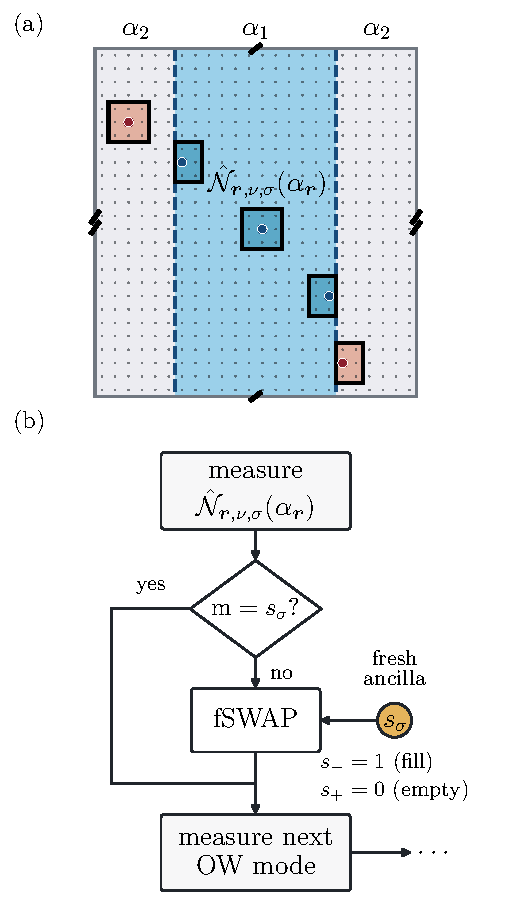
\includegraphics[width=0.75\columnwidth]{Figure_01_schematic.pdf}
    \caption{\newtext{\textbf{Domain-wall geometry and adaptive circuit.} (a) Periodic geometry with $\alpha_{\boldsymbol r}=\alpha_1$ in the central slab and $\alpha_2$ in the trivial exterior. Matching marks identify opposite boundaries. Salmon and blue windows show exterior and slab OW supports; dots mark their centers. Bulk supports contain $3\times3$ cells; interface supports are clipped and renormalized. (b) An occupation measurement returns the Born outcome $\mathrm m$. If $\mathrm m=s_\sigma$, correction is bypassed; otherwise an fSWAP with a fresh ancilla restores $s_-=1$ or $s_+=0$. The branches rejoin and the procedure repeats for subsequent OW modes.}}
    \label{fig:Geometry}
    \label{fig:Circuit}
\end{figure}

\subsection{Adaptive circuit}
\label{sec:Circuit}
\label{sec:FermionCounting}
\newtext{The circuit corrects undesired OW occupations by a fermionic SWAP (fSWAP) with an ancillary mode, following Ref.~\cite{BhuiyanPanJian2026}. Here, each correction uses a fresh ancilla with the target occupation: filled for a lower-band mode and empty for an upper-band mode. Every correction therefore succeeds, unlike the finite-bath protocol, where success depends on the ancillary occupation. Discarding the ancilla reduces the correction to single-fermion gain or loss,}
\begin{align}
    \braa{0}_a\fSWAP(\hat\chi_{\bfr,\nu,-},\hat d)\big(\hat\Id-\hat{\mc N}_{\bfr,\nu,-}\big)\kett{1}_a&=\hat\chi^\dagger_{\bfr,\nu,-},\nonumber\\
    \braa{1}_a\fSWAP(\hat\chi_{\bfr,\nu,+},\hat d)\,\hat{\mc N}_{\bfr,\nu,+}\kett{0}_a&=\hat\chi_{\bfr,\nu,+},
    \label{eq:GainLoss}
\end{align}
\newtext{where $\hat d$ denotes the fresh ancillary mode. The fSWAP expression, fermionic ordering convention, and derivation are given in Appendix~\ref{app:FermionCounting}. The effective operations remain Gaussian but do not conserve the physical particle number.} In the composite system, both the occupation measurement and the fSWAP gate conserve the total charge, so the dynamics has a strong $U(1)$ symmetry. After the ancillas are discarded, only a weak $U(1)$ symmetry remains: the Born-averaged channel commutes with $U(1)$ rotations, but individual Kraus operators do not~\cite{BucaProsen2012,AlbertJiang2014}.

\newtext{Monitored fermion gain and loss is known as fermion counting~\cite{StarchlFischerSieberer2025,KloiberTollingerSieberer2026,SoaresLeGalSchiro2025}. Our measurement-and-feedforward step is equivalent to single-mode fermion counting run to completion, as shown in Appendix~\ref{app:FermionCounting}.}

\newtext{Figure~\ref{fig:Circuit}(b) summarizes one elementary step.} For brevity, we write $i=(\bfr,\nu)$ and denote the truncated lower- and upper-band OW modes by $\hat\chi_{i,-}$ and $\hat\chi_{i,+}$. A measurement of $\hat{\mc N}_{i,\sigma}$ returns $\mathrm{m}=1$ with Born probability $\langle\hat{\mc N}_{i,\sigma}\rangle$ and $\mathrm{m}=0$ otherwise, where the expectation value is taken in the conditioned state just before the measurement.



By Eq.~\eqref{eq:GainLoss}, each elementary step therefore acts on the physical system alone through a pair of Kraus operators,
\begin{align}
    \hat K_{i,-}(\mathrm{m})&=\mathrm{m}\,\hat{\mc N}_{i,-}+(1-\mathrm{m})\,\hat\chi^\dagger_{i,-},
    \label{eq:KrausLower}\\
    \hat K_{i,+}(\mathrm{m})&=(1-\mathrm{m})\big(\hat\Id-\hat{\mc N}_{i,+}\big)+\mathrm{m}\,\hat\chi_{i,+},
    \label{eq:KrausUpper}
\end{align}
for lower- and upper-band modes, respectively. For a lower-band mode, the outcome $\mathrm{m}=1$ leaves the state unchanged and the outcome $\mathrm{m}=0$ is followed by gain. For an upper-band mode, the outcome $\mathrm{m}=0$ leaves the state unchanged and the outcome $\mathrm{m}=1$ is followed by loss. Both pairs are Gaussian and satisfy $\sum_{\mathrm{m}=0,1}\hat K^\dagger_{i,\sigma}(\mathrm{m})\hat K_{i,\sigma}(\mathrm{m})=\hat\Id$. In words, $\hat K_{i,-}$ always leaves the lower-band mode filled and $\hat K_{i,+}$ always leaves the upper-band mode empty, regardless of the outcome.

One cycle visits every unit cell and applies the four updates $(A,+)$, $(A,-)$, $(B,+)$, $(B,-)$ at each. Since truncated OW modes centered on nearby unit cells overlap, their measurements generally do not commute, so the order within a cycle is part of the protocol. We use a raster order, increasing $y$ at fixed $x$ before advancing to the next column, so that a cycle contains $4N_xN_y$ elementary steps. Note that measurements with nonoverlapping supports commute, so a cycle can also be organized into a system-size-independent number of layers of mutually commuting operations, as in Ref.~\cite{BhuiyanPanJian2026}. We expect the universal properties studied below not to depend on this choice.
\GPT{Disjoint-support operations commute, but regrouping a prescribed raster word into a bounded number of layers also changes the order of overlapping operations. Distinguish finite operation range from a demonstrated finite-depth implementation of this particular schedule.}


For a measurement record $\rec$ accumulated over $t$ cycles, the conditioned state is $\hat\rho_{\rec}(t)=\hat V_{\rec}\hat\rho_0\hat V_{\rec}^\dagger/p(\rec)$, where $\hat V_{\rec}$ is the ordered product of all Kraus operators along the record and $p(\rec)=\Tr[\hat V_{\rec}\hat\rho_0\hat V_{\rec}^\dagger]$ is its Born probability. The object of interest is the ensemble $\{p(\rec),\hat\rho_{\rec}(t)\}$. Following Ref.~\cite{BhuiyanPanJian2026}, we refer to quantities that require the resolution of individual records, such as entanglement entropies, as \emph{trajectory resolved}. We refer to quantities that follow from the averaged state $\overline{\hat\rho}(t)=\sum_{\rec}p(\rec)\hat\rho_{\rec}(t)$ as \emph{trajectory averaged}. We denote the Born-weighted average of a trajectory-resolved quantity by an overline. For nonlinear quantities, such as the entanglement entropy, the quantity is always evaluated in each trajectory before the average is taken. Hence, $\overline{S}$ denotes the average entropy of the conditioned states, not the entropy of $\overline{\hat\rho}$.

Since every operation is Gaussian, each conditioned state remains Gaussian and is fully characterized by its two-point function
\begin{equation}
    \claudeadd{G_{ij}=\Tr\!\big(\hat\rho\,\hat c_j^\dagger\hat c_i\big),}
    \label{eq:TwoPoint}
\end{equation}
where $i,j$ now run over unit cells and orbitals. With this ordering, \claudeadd{$G$} for a pure Gaussian state is the projector onto its occupied single-particle states. In general, \newtext{the eigenvalues of $G$} lie in $[0,1]$. Writing \claudeadd{$P_j=W_jW_j^\dagger$} for the single-particle projector onto the measured OW mode, $Q_j=\Id-P_j$, \newtext{with $W_j$ the column vector of its creation wavefunction,} the Born probability of outcome $\mathrm m$ is \claudeadd{$p_j(1)=n_j$ and $p_j(0)=1-n_j$, with $n_j=\operatorname{tr}(P_jG)$ the mean occupation of the measured mode}. The conditional update, including the feedforward to the target occupation $s_-=1$ or $s_+=0$, is~\cite{bravyi2004lagrangian,BhuiyanPanJian2026}
\begin{equation}
    \claudeadd{G'=Q_jGQ_j-\eta_{\mathrm m}\,\frac{Q_jGP_jGQ_j}{p_j(\mathrm m)}+s_\sigma P_j,}
    \label{eq:CovarianceUpdate}
\end{equation}
\claudeadd{where $\eta_{\mathrm m}=2\mathrm m-1$. Because $P_j$ has rank one, Eq.~\eqref{eq:CovarianceUpdate} requires no matrix inversion: its only denominator is the Born probability $p_j(\mathrm m)$, which is nonzero for every outcome that occurs.} We simulate the circuit by iterating Eq.~\eqref{eq:CovarianceUpdate}.

\claudeadd{With this ordering, no transposes appear; Ref.~\cite{BhuiyanPanJian2026} used the transposed convention $G_{ij}=\langle\hat c_i^\dagger\hat c_j\rangle$.}

\FloatBarrier
\section{Dynamical Chiral Domain-Wall Modes}
\label{sec:Results}

In the following, we numerically study the adaptive circuit of Sec.~\ref{sec:Model} with hard domain walls. Unless stated otherwise, we use $N_x=20$ with interfaces at $x=5$ and $15$, $\alpha_2=30$, and truncation range $w=1$. We take $\alpha_1=1$ inside the slab, where the target state has $\mc C=1$, and use $\alpha_1=3$ as a trivial control. In Ref.~\cite{BhuiyanPanJian2026}, we found that the degrees of freedom near such a domain wall purify algebraically slowly, and we anticipated nonequilibrium analogs of chiral edge modes there. In this section, we characterize these modes.
{\color{blue}
Throughout this section, an overline denotes the Born-rule average over measurement trajectories, estimated using $S=100$ independent trajectories per parameter set unless stated otherwise. For subsystem observables, we also average over all translated origins $y_0$ along the periodic $y$ direction, first within each trajectory and then over trajectories. Entropies, charge variances, and other nonlinear observables are evaluated for each trajectory and subsystem position before averaging. Coordinates within a translated subsystem are reported relative to its origin, $\delta y=(y-y_0)\bmod N_y$. Additional spatial averages and exceptions are stated where they enter.

\claudecom{Narrative: with the state-preparation framing, the cleaner order is bulk $\to$ wall correlations $\to$ entanglement and charge $\to$ per-wall entropy $\to$ chirality, and only then purification. The purification section would then read as the cost of preparing the walls rather than as a detour before the main result. Optional, but it also matches your introduction's ``Finally, we study slow purification''.} We begin with the topology of the prepared bulk and the slow purification of its boundaries. We then characterize the pure boundary states through correlations, entanglement, charge fluctuations, and their restricted spectra, before resolving the two walls and their modular propagation. Finally, we compare these trajectory-resolved signatures with the outcome-averaged channel.
}

{\color{blue}
\subsection{Bulk preparation in the domain-wall geometry}
\label{sec:BulkTopology}

We first verify that the finite-range circuit prepares the intended bulk phase inside the slab. We evolve random pure half-filled states on square systems, $N_x=N_y=L$, with $L=20,30,40$, for 40 cycles. Following Ref.~\cite{Kitaev2006}, we partition a disk within the slab into three counterclockwise sectors $A,B,C$ [Fig.~\ref{fig:BulkTopology}(a)] and evaluate
\begin{align}
    \mc C_G=12\pi\operatorname{Re}\!\left\{\ii\left[\operatorname{tr}(P_{CA}P_{AB}P_{BC})\right.\right.\nonumber\\
    \left.\left.{}-\operatorname{tr}(P_{AC}P_{CB}P_{BA})\right]\right\},
    \label{eq:KitaevChern}
\end{align}
where \claudeadd{$P=G$} and $P_{XY}$ is its block with rows in $X$ and columns in $Y$. Both orbitals of a cell belong to the same sector. We take radius $R=0.2L$ and center $x_0=L/2$, and average over ten randomly sampled transverse centers within each trajectory before taking the trajectory average.

Figure~\ref{fig:BulkTopology}(c) shows that $\overline{\mc C_G}$ approaches one within a few cycles. At cycle 40, its deviation from one decreases from approximately $2.4\times10^{-3}$ at $L=20$ to $1.4\times10^{-5}$ at $L=40$. Thus the shortest OW range used here already prepares a bulk state with the target Chern number on the accessible sizes.

To resolve the topology in space, we also compute the local Chern marker introduced by Bianco and Resta~\cite{BiancoResta2011}, with the overall sign chosen to match Eq.~\eqref{eq:ChernNumber},
\begin{equation}
 C(\bfr)=\sum_\mu\operatorname{Re}\!\left[2\pi\ii\big(PXPYP-PYPXP\big)_{\bfr\mu,\bfr\mu}\right],
 \label{eq:LocalMarker}
\end{equation}
where $X,Y$ are the finite-sample position matrices. The mean marker is close to one in the slab interior. Figure~\ref{fig:BulkTopology}(b) displays $\tanh[\overline{C(\bfr)}]$ on a color scale from $-1$ to $1$ to compress the large seam contribution; the transformation is applied after trajectory averaging. \claudedel{It differs from the finite-disk estimator: ordinary position coordinates on a periodic sample introduce a seam, and the marker sums to zero over the entire finite lattice. The compensating seam contribution therefore does not indicate a trivial slab.}\claudeadd{On a periodic lattice, the position operators jump at a seam, and the marker sums to zero over the whole lattice. The compensating contribution at the seam is therefore an artifact of the coordinates, not a sign of a trivial slab.}
}

\begin{figure}[!htbp]
    \centering
    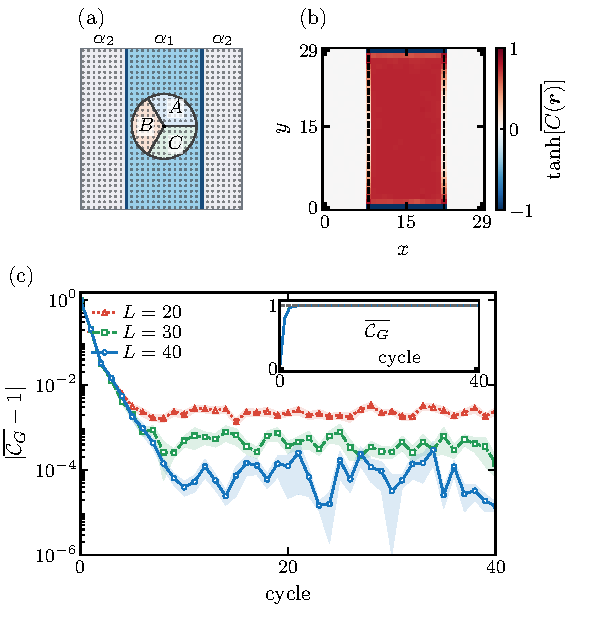
\includegraphics[width=\columnwidth]{Figure_03_bulk_topology.pdf}
    \caption{\newtext{\textbf{Bulk topology in the domain-wall geometry.} (a) A $30\times30$ lattice with interfaces at $x=8,22$ and a three-sector disk of radius $R=6$. The drawn transverse center is representative. (b) Local Chern marker [Eq.~\eqref{eq:LocalMarker}] at $L=30$, cycle 40, displayed as $\tanh[\overline{C(\bfr)}]$ after averaging $S=100$ independent trajectories. The bounded color scale compresses the periodic-coordinate seam contribution. (c) $|\overline{\mc C_G}-1|$ for $L=20,30,40$, with the untransformed $\overline{\mc C_G}$ in the inset. Each cycle averages ten randomly chosen disk centers per trajectory, then $S=100$ independent trajectories. Shading is one trajectory SEM. All ensembles start from random pure half-filled states and use $\alpha_1=1$, $\alpha_2=30$, and $w=1$.}}
    \label{fig:BulkTopology}
\end{figure}

{\color{blue}
\subsection{Slow purification and gapless Lyapunov modes}
\label{sec:Purification}

Having established the bulk topology, we ask how the circuit removes the entropy of a mixed initial state. The bulk and boundary need not purify on the same time scale. For each trajectory, the full-system entropy and its spatial contour are
\begin{align}
 S_{\rec}(t)&=\sum_j h(\nu_j),\nonumber\\
 s_{\rec}(\bfr,t)&=\sum_\mu[h(G_{\rec}(t))]_{\bfr\mu,\bfr\mu},
 \label{eq:BinaryEntropy}
\end{align}
where $h(u)=-u\log u-(1-u)\log(1-u)$ and $\nu_j$ are occupation eigenvalues. We sum the contour over $y$ to obtain the column entropy $s_x(t)$.

Starting from the maximally mixed state, the trivial control $\alpha_1=3$ loses its entropy within about ten cycles, whereas the $\alpha_1=1$ state purifies slowly over the simulated window [Fig.~\ref{fig:Purification}(a)]. The residual entropy is concentrated at the two walls; columns deep in the trivial exterior purify rapidly [Fig.~\ref{fig:Purification}(b)]. The late plateau of the trivial control reflects the numerical entropy floor.

The purification probes the spectrum of the trajectory evolution operator. For a maximally mixed initial state, its positive part determines the conditioned state,
\begin{equation}
 \hat\rho_{\rec}(T)=\frac{\hat V_{\rec}(T)\hat V_{\rec}^\dagger(T)}
 {\Tr[\hat V_{\rec}(T)\hat V_{\rec}^\dagger(T)]}
 \propto e^{-2T\hat{\mathcal H}_{\rec}(T)},
 \label{eq:PurificationKrausProduct}
\end{equation}
where $\hat{\mathcal H}_{\rec}=\sum_{ij}[h_{\rec}]_{ij}\hat c_i^\dagger\hat c_j+\mathrm{const.}$ is the effective Gaussian Hamiltonian. Its eigenvalues encode logarithms of the singular values of $\hat V_{\rec}$, up to an additive constant. The single-particle matrix $h_{\rec}$ and the correlation matrix have the same eigenvectors, with
\begin{equation}
 G_{\rec}(T)=\big[\mathbf{1}+e^{2T h_{\rec}(T)}\big]^{-1}.
 \label{eq:PurificationFermiFunction}
\end{equation}
The occupation eigenvalues therefore give the finite-time single-particle Lyapunov rates and their smallest magnitude,
\begin{equation}
 \gamma_j(T)=\frac{1}{2T}\log\frac{1-\nu_j(T)}{\nu_j(T)},\qquad
 \Delta_{\rec}(T)=\min_j|\gamma_j(T)|.
 \label{eq:LyapunovFromOccupations}
\end{equation}
A nearly pure mode contributes entropy $(1+2T|\gamma_j|)e^{-2T|\gamma_j|}$ to leading order. Modes near zero thus retain entropy longest, and their eigenvector densities determine where that entropy resides. A limiting gap $\Delta>0$ gives an exponential entropy rate $2\Delta$ at fixed size; a closing gap removes a size-independent rate. This connection between topological Lyapunov boundary modes and slow purification was developed in Ref.~\cite{XiaoKawabata2026}; here we examine it under Born-rule dynamics without postselection.

The same trajectory operator also acts on a pure initial state, which remains pure after conditioning. Along a fixed record, its singular values weight the components of the initial state in the right singular-vector basis; the corresponding left singular vectors form the output. Relative singular values therefore describe dynamical filtering even when the state has no entropy to lose, with the initial overlaps selecting the contributing components. In that case the full-system occupations are already zero or one, so Eq.~\eqref{eq:LyapunovFromOccupations} cannot extract finite rates from the pure-state correlation matrix. The mixed-state purification experiment exposes this operator spectrum directly. The singular-support qualifications and entropy asymptotics are given in Appendix~\ref{app:Lyapunov}.

The independent size sweep in Fig.~\ref{fig:Lyapunov}(a) gives $\overline\Delta\propto N_y^{-z}$ with $z=1.08\pm0.05$ at $T=2N_y$. The decrease is consistent with slow boundary modes, although a finite-time size scan alone does not determine the infinite-time Lyapunov gap. We locate the slowest mode by taking the normalized eigenvector $|\phi_{\min}\rangle$ whose occupation is closest to $1/2$, and compute
\begin{equation}
 p_{\min}(x,y)=\sum_\mu|\langle x,y,\mu|\phi_{\min}\rangle|^2.
 \label{eq:SlowestModeDensity}
\end{equation}
Its mean density lies on the walls [Fig.~\ref{fig:Lyapunov}(b)]. Either wall can host the slowest mode in an individual trajectory, so averaging covers both walls. These spatial profiles connect the residual entropy to boundary-localized slow modes.
}

\begin{figure}[!htbp]
    \centering
    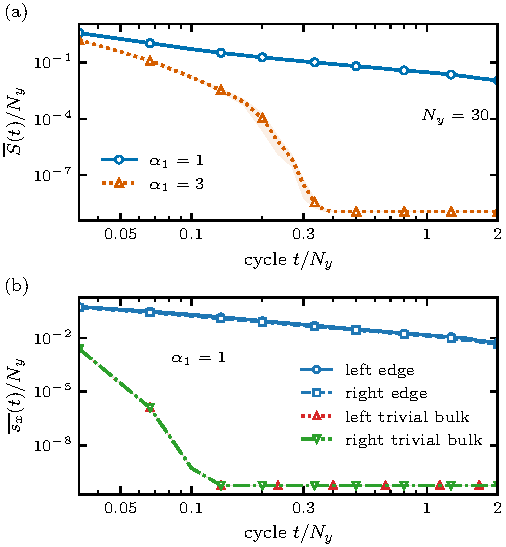
\includegraphics[width=\columnwidth]{Figure_04_purification.pdf}
    \caption{\newtext{\textbf{Slow purification at the domain walls.} (a) Mean entropy per unit length at $N_y=30$ for $\alpha_1=1,3$. (b) Column entropy at $\alpha_1=1$ on the walls, $x=5,15$, and in the trivial exterior, $x=2,18$. Both panels start with the full system maximally mixed and use $S=100$ independent trajectories evolved for 60 cycles. Bands are one trajectory SEM; the trivial entropy plateau is a numerical floor.}}
    \label{fig:Purification}
\end{figure}

\begin{figure}[!htbp]
    \centering
    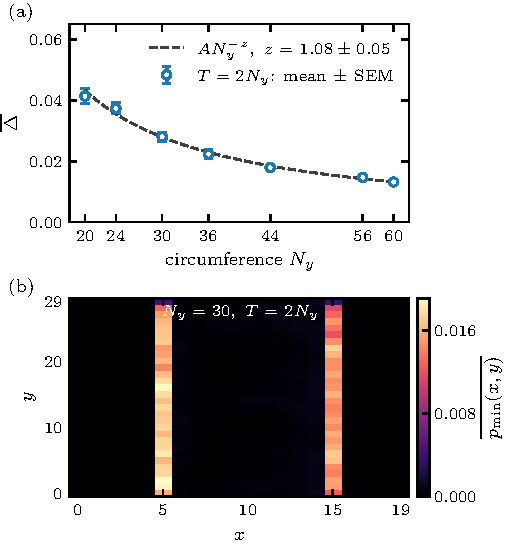
\includegraphics[width=\columnwidth]{Figure_04_lyapunov.pdf}
    \caption{\newtext{\textbf{Finite-time Lyapunov gap and boundary modes.} (a) Mean gap at $T=2N_y$ for $N_y=20,24,30,36,44,56,60$; the dashed line is an SEM-weighted fit over all seven sizes, with $z=1.08\pm0.05$. The slab is initially maximally mixed and the decoupled exterior is pure. (b) Mean density of the unique slowest mode at $N_y=30$, $T=60$, starting with the full system maximally mixed. Both ensembles use $\alpha_1=1$ and $S=100$ independent trajectories. Each gap and mode density is evaluated within a trajectory before averaging; error bars are one trajectory SEM.}}
    \label{fig:Lyapunov}
\end{figure}

\subsection{Algebraic correlations along the walls}
\label{sec:Correlations}

{\color{blue}
We start with the pure states prepared by the circuit. Unless stated otherwise, we evolve random pure half-filled states for $2N_y$ cycles and average over $100$ independent trajectories per system size. The most direct signature of gapless wall modes is in the correlations along the walls. Within each pure Gaussian trajectory, the connected density correlation between distinct modes is $\langle\hat n_i\hat n_j\rangle_c=-|G_{ij}|^2$. The negative sign expresses anticorrelated occupation fluctuations; the joint occupation probability itself remains nonnegative. We study their positive magnitude through the squared two-point function along $y$,
\begin{equation}
    C_G(x,r_y)=\frac{1}{2N_y}\sum_{y,\mu,\nu}\big|G_{(x,y,\mu),(x,y+r_y,\nu)}\big|^2,
    \label{eq:SquaredCorrelator}
\end{equation}
together with its average $C_G^{\rm av}(r_y)$ over $x$. The connected density correlation is evaluated within each trajectory before averaging; it is not the connected correlation of the trajectory-averaged state. We average over trajectories after squaring. For distances along the periodic direction, we use the chord length $D(\ell)=(N_y/\pi)\sin(\pi\ell/N_y)$ throughout, leaving its dependence on the circumference implicit. Its argument is the separation $r_y$ here and the strip width $A_y$ below. For a free chiral fermion, $\overline{C_G}\propto D(r_y)^{-2}$.
}

\begin{figure}[!htbp]
    \centering
    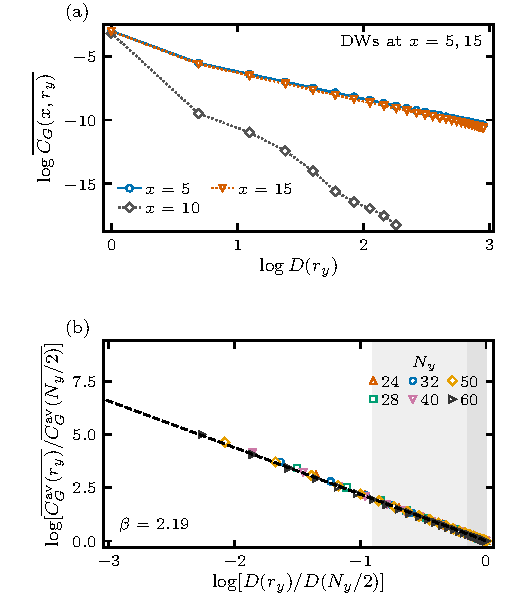
\includegraphics[width=\columnwidth]{Figure_05_correlations.pdf}
    \caption{\newtext{\textbf{Algebraic correlations on the walls.} (a) Column-resolved correlations at $\alpha_1=1$, $N_y=60$, for $x=5,10,15$. (b) Antipodally normalized correlations for $N_y=24,28,32,40,50,60$, displaying $r_y\geq2$. The dashed line is a joint power-law fit over $8\leq r_y\leq N_y/2$, with equal total weight per size and $\beta\approx2.19$. \claudecom{General note on captions: many carry estimator details (``transformed through the absolute value'', ``translated cuts are correlated observations'', ``the gap is dimensionless''). Keep panel descriptions and parameters, and move statistics conventions to one sentence at the start of Sec.~\ref{sec:Results}, which you already have.} Gray shading marks the fit-window range. The data use $S=100$ independent random-pure half-filled trajectories per case, observed after $2N_y$ cycles; spatial averaging precedes trajectory averaging, and the logarithm is taken last. Values below $10^{-8}$ are omitted from (a).}}
    \label{fig:Correlations}
\end{figure}

\newtext{The column-resolved correlations in Fig.~\ref{fig:Correlations}(a) show that the long-range part comes from the wall columns, while the correlations at the slab center decay rapidly.} Normalizing by the value at the antipodal distance collapses all circumferences onto a single power law [Fig.~\ref{fig:Correlations}(b)] with exponent $\beta\approx2.2$, slightly above the free-chiral-fermion value $\beta=2$ at these system sizes. \newtext{These data support critical, one-dimensional wall correlations, while correlations in the slab interior remain short ranged.} In the following sections, we identify these modes as chiral.

\subsection{Entanglement and charge fluctuations along the walls}
\label{sec:Entanglement}

{\color{blue}
We now quantify the wall modes using entanglement and charge fluctuations, with $N_y=30,35,\ldots,60$. For each trajectory, we consider the full-width strip
\begin{equation}
    A(y_0,A_y)=[0,N_x)\times[y_0,y_0+A_y)\pmod{N_y},
    \label{eq:Strip}
\end{equation}
which crosses both walls. The restriction $G_A$ of the two-point function to $A$ has eigenvalues $\nu_a\in[0,1]$, which determine both the von Neumann entropy $S\equiv S_1$ and the charge variance $F$ of $A$~\cite{KlichLevitov2009,SongFlindtRachel2011},
\begin{equation}
    S(A)=\sum_a h(\nu_a),
    \qquad
    F(A)=\sum_a\nu_a(1-\nu_a),
    \label{eq:EntropyVariance}
\end{equation}
\newtext{with $h$ defined in Eq.~\eqref{eq:BinaryEntropy}.}
Here, $F(A)$ measures the charge fluctuations within a single conditioned state, not the variation of its mean charge between records.
}

{\color{blue}
\newtext{A useful comparison is a pair of spatially separated free chiral branches.} For an interval on a circle, conformal invariance replaces the interval length by $D(A_y)$. A single chiral branch with central charge $c_w$ contributes $(c_w/6)\log D(A_y)$ to the entropy~\cite{CalabreseCardy2004}, and a charge-one chiral $U(1)$ current at level $k_w$ contributes $(k_w/2\pi^2)\log D(A_y)$ to the charge variance~\cite{DiFrancescoMathieuSenechal1997}. The full-width strip intersects both walls, whose contributions add despite their opposite propagation directions. Hence, we expect
\begin{align}
    \overline{S}(A_y)&=\frac{c}{3}\log D(A_y)+\text{const.},\nonumber\\
    \overline{F}(A_y)&=\frac{k}{\pi^2}\log D(A_y)+\text{const.},
    \label{eq:CFTScaling}
\end{align}
\newtext{Here $c\equiv c_1$ denotes the von Neumann coefficient, with $c=k=1$ for a charge-one complex fermion on each wall.} \newtext{The overlines include the average over $y_0$ within each trajectory.} To compare circumferences, we subtract from each curve its value at the half-strip $A_y^\star=\lfloor N_y/2\rfloor$, which removes the nonuniversal constants. The horizontal coordinate is then $\log[D(A_y)/D(A_y^\star)]$.
}

{\color{blue}
\begin{figure}[!htbp]
    \centering
    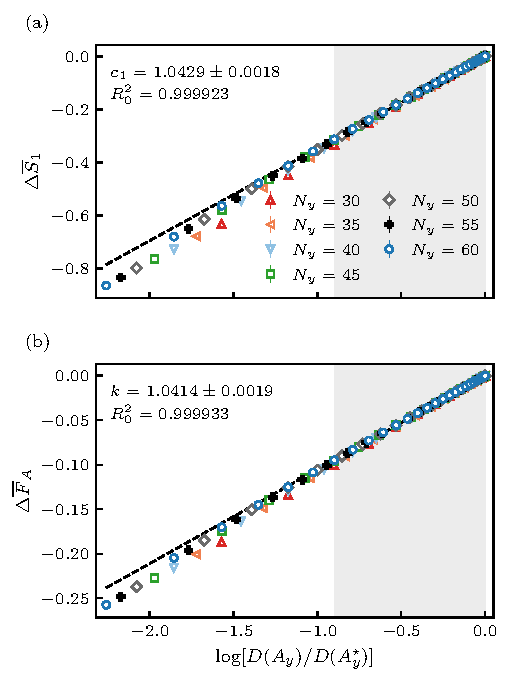
\includegraphics[width=\columnwidth]{Figure_06_entropy_charge.pdf}
    \caption{\newtext{\textbf{Entanglement and charge fluctuations.} (a) Mean strip entropy and (b) charge variance for $N_y=30,35,\ldots,60$, shifted by their values at $A_y=\lfloor N_y/2\rfloor$. Each case uses $S=100$ independent random-pure half-filled trajectories after $2N_y$ cycles, with all strip origins averaged within each trajectory. Dashed lines are joint fits to Eq.~\eqref{eq:CFTScaling} over $8\leq A_y\leq\lfloor N_y/2\rfloor$ (shaded). The point $A_y=1$ is excluded from display only. The fits and their trajectory-based uncertainties retain correlations between strip widths.}}
    \label{fig:EntropyCharge}
\end{figure}
}



{\color{blue}
Figure~\ref{fig:EntropyCharge} shows that both observables follow the logarithmic chord-length dependence. The fitted coefficients are close to $c\simeq k\simeq1.04$, with a common excess over one at these sizes. Their agreement is consistent with charge-one free-fermion branches\claudedel{, but does not by itself identify the conditioned states with an equilibrium ground state}\claudeadd{, since entanglement and charge fluctuations are governed by the same free-fermion correlations}.

The restricted spectrum gives a complementary view of this scaling. \claudeadd{Write $\lambda_a=2\nu_a-1$, where $\nu_a$ are the eigenvalues of $G_A$.} The corresponding single-particle entanglement energies are
\begin{equation}
 \varepsilon_a=\log\frac{1-\nu_a}{\nu_a}
 =\log\frac{1-\lambda_a}{1+\lambda_a}.
 \label{eq:EntanglementEnergies}
\end{equation}
For the half-strip at $N_y=32$, the full occupation distribution is strongly concentrated near $\lambda=\pm1$ [Fig.~\ref{fig:Spectrum}(a)]. These nearly pure modes contribute little entropy per mode. Panel (b) resolves the partially occupied modes by restricting to $|\lambda|\leq0.99$ and normalizing the energy histogram to unit area within this window. This cutoff is equivalent to $0.005\leq\nu\leq0.995$, hence $|\varepsilon|\leq\log(0.995/0.005)=\log199\simeq5.29$\claudedel{; the energy-window endpoint is set by the cutoff}. For $\alpha_1=1$, the distribution extends through zero entanglement energy with finite density, consistent with gapless boundary modes. In contrast, $\alpha_1=3$ shows a pronounced gap-like depletion around zero. Sparse near-zero levels remain in the pooled trivial distribution, so this depletion does not establish a strict entanglement gap. Modes in the latter need not be dynamical slow modes: a reduced state can have partially occupied entanglement levels even when its spatial entanglement obeys an area law.

Normalization removes the total number of modes, so we separately count
\begin{align}
 N_{0.99}(A_y)&=\sum_a\mathbf1_{\{|\lambda_a|\leq0.99\}},\nonumber\\
 \overline N_{0.99}(A_y)&\simeq a+b\log D(A_y).
 \label{eq:WindowCount}
\end{align}
Here $\mathbf1_{\{\cdots\}}$ is the indicator of the spectral window. Figure~\ref{fig:Spectrum}(c) shows logarithmic growth for $\alpha_1=1$, with $b=1.187\pm0.013$ over $5\leq A_y\leq16$. A spectral density proportional to $\log D(A_y)$ over the entropy-relevant energies gives logarithmic entropy and charge variance, since each is a sum of a fixed function of $\varepsilon_a$. This mechanism also appears in the equilibrium free-fermion analysis of Ref.~\cite{EislerPeschel2010}, Sec.~V. Here the logarithmic count provides a consistent spectral interpretation of Fig.~\ref{fig:EntropyCharge}; its window-dependent slope is not itself a central charge.
}

\begin{figure}[!htbp]
    \centering
    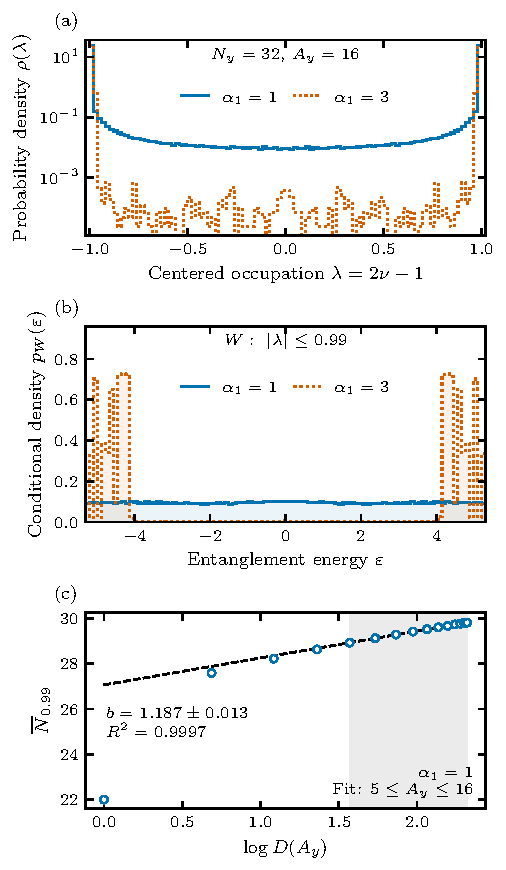
\includegraphics[width=\columnwidth]{Figure_07_entanglement_spectrum.pdf}
    \caption{\newtext{\textbf{Restricted spectra and mode count.} Hard-wall states at $N_x=20$, $N_y=32$, cycle 64, from $S=100$ independent random-pure half-filled trajectories per $\alpha_1=1,3$. (a) Full centered-occupation histogram, normalized to unit area. (b) Conditional unit-area energy density for $|\lambda|\leq0.99$, in 101 equal bins on $[-\log199,\log199]$. The central depletion at $\alpha_1=3$ contrasts with the finite near-zero density at $\alpha_1=1$. Both histograms pool all 32 translated half-strips per trajectory. The retained totals are 95,398 and 83,326 for $\alpha_1=1,3$. (c) Raw mean window count for $\alpha_1=1$, averaging origins within each trajectory. Bars are one trajectory SEM; the dashed fit uses $5\leq A_y\leq16$ (shaded), while all widths are displayed. \claudedel{Translated cuts are correlated observations, not additional trajectories.}}}
    \label{fig:Spectrum}
\end{figure}

\claudecom{Agree with GPT. Since the slope $b$ depends on the window and is not universal, consider moving the window count to the appendix and keeping only panels (a,b) in the main text as the gapless-versus-gapped entanglement spectrum, which is the Li--Haldane-type message~\cite{LiHaldane2008}.} \GPT{The histogram at one width does not establish that the coefficient of the logarithm in the unnormalized spectral density is energy independent. The count also has a substantial constant background; a quantitative entropy coefficient cannot be inferred from its slope alone.}

{\color{blue}
We next check how the entropy coefficient approaches its late-time value. For each size and cycle, we fit the mean strip entropy to Eq.~\eqref{eq:CFTScaling}, with a free intercept over $8\leq A_y\leq N_y/2$, and write $c_{\rm eff}=3m_1$ for the fitted slope. Figure~\ref{fig:Ceff}(a) in Appendix~\ref{app:MutualInformation} shows the approach from random pure initial states. The coefficient decreases toward a value close to one, while the inset resolves the remaining deviation. The independent endpoint ensemble in Fig.~\ref{fig:Ceff}(b) shows that the excess over one decreases overall with circumference, with visible finite-size variation. \claudedel{Neither panel is an extrapolation establishing an exact equilibrium coefficient. Together with the charge fluctuations and spectral count, they support logarithmic boundary entanglement in the conditioned states.}\claudeadd{Together with the charge fluctuations, these results support logarithmic boundary entanglement in the conditioned states, with a coefficient approaching one as the circumference grows.}
}



{\color{blue}
Appendix~\ref{app:MutualInformation} gives two additional spatial checks: the mean entropy contour distinguishes the critical walls from the trivial control, and the mutual information between antipodal strips tracks the loss of the wall signal as $\alpha_1$ increases.
}

{\color{blue}\subsection{Entropy carried by each wall}
\label{sec:ChiralCentralCharge}}

The full-width strip only reveals the sum of the two walls. A single chiral branch with left- and right-moving central charges $c_L$ and $c_R$ contributes \newtext{$(c_L+c_R)\log D(A_y)/6$} to the entropy of an interval~\cite{CalabreseCardy2004,CastroDetournayIqbalPerlmutter2014}, i.e., half of the familiar nonchiral coefficient $c/3$. The nontrivial statement is therefore that the coefficient $c\approx1$ of Sec.~\ref{sec:Entanglement} splits in real space into one half from each wall. Note that a nonchiral wall with a single Dirac fermion would give the full coefficient on one wall.

{\color{blue}
To resolve the two walls, we use the entanglement contour $s\equiv s_1$~\cite{BhuiyanPanJian2026}
\begin{equation}
    s(\bfr;A)=\sum_\mu\langle\bfr,\mu|\,h(G_A)\,|\bfr,\mu\rangle,
    \label{eq:Contour}
\end{equation}
which distributes $S(A)$ over the sites of $A$. For a half-strip, the averaged contour is concentrated on the two wall columns, apart from area-law contributions along the cuts inside the slab, while the trivial exterior contributes almost nothing.
We then average the contour of each trajectory over the strip position $y_0$, with coordinates $\delta y=y-y_0$ measured from the start of the strip, and integrate it over a two-column window adjacent to each wall,
\begin{align}
    \overline{S}^{\rm wall}_{L}(A_y)&=\sum_{x=5}^{6}\sum_{\delta y=0}^{A_y-1}\overline{s}(x,\delta y),\nonumber\\
    \overline{S}^{\rm wall}_{R}(A_y)&=\sum_{x=14}^{15}\sum_{\delta y=0}^{A_y-1}\overline{s}(x,\delta y),
    \label{eq:WallEntropy}
\end{align}
\newtext{Fitting the half-strip-subtracted curves against $\log[D(A_y)/D(A_y^\star)]$ gives the slope $m_w$ and entropy weight $3m_w$. If the wall carries a single chiral branch, its central charge has magnitude $|c_-^{(w)}|=6m_w$, where $c_-=c_R-c_L$. Entropy alone measures $c_L+c_R$ and does not determine chirality.}
}

\begin{figure}[!htbp]
    \centering
    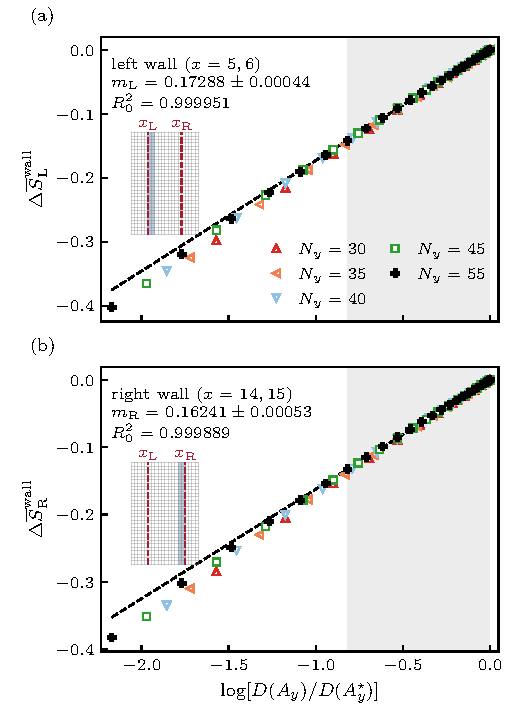
\includegraphics[width=\columnwidth]{Figure_09_wall_entropy.pdf}
    \caption{\newtext{\textbf{Entropy carried by each wall.} Entanglement contour integrated over (a) $x=5,6$ and (b) $x=14,15$, for $N_y=30,35,40,45,55$. Each case uses $S=100$ independent random-pure trajectories after $2N_y$ cycles. Contours are averaged over all translated strips within each trajectory before trajectory averaging, and anchored at $A_y=\lfloor N_y/2\rfloor$. Dashed lines are joint fits over $8\leq A_y\leq\lfloor N_y/2\rfloor$ (shaded), with equal total weight per size and trajectory-based uncertainties including correlations between widths. Insets mark the integrated columns. The point $A_y=1$ is omitted from display only.}}
    \label{fig:WallEntropy}
\end{figure}

\newtext{As shown in Fig.~\ref{fig:WallEntropy}, the two windows contribute entropy weights $3m_L\approx0.52$ and $3m_R\approx0.49$. Their sum, approximately $1.01$, accounts for most of the full-strip coefficient, with the remaining contour weight outside these windows. Each contribution is close to the half-unit weight expected for a single chiral branch with $|c_-|=1$. \claudecom{This is your sharpest evidence that each wall carries exactly one chiral branch, since a nonchiral wall would carry the full coefficient. It is underplayed relative to the spectral count; the abstract rewrite now leads with it.} These entropy weights do not determine the propagation direction. We turn to that question next.}

{\color{blue}
\subsection{Opposite chiralities from modular evolution}
\label{sec:ModularEvolution}

To probe the handedness of the wall modes, we use the modular Hamiltonian of a half-cylinder containing all columns and $N_y/2$ consecutive rows. With the correlator convention of Eq.~\eqref{eq:TwoPoint}, define
\begin{equation}
 h_A=\log[(\Id_A-G_A)G_A^{-1}]=-2\arctanh(2G_A-\Id_A).
 \label{eq:ModularHamiltonian}
\end{equation}
The reduced state is $\hat\rho_A\propto e^{-\hat K_A}$, where \claudeadd{$\hat K_A=\sum_{ij}[h_A]_{ij}\hat c_i^\dagger\hat c_j$.} Thus a coefficient vector of an annihilation mode, $\hat\chi_\varphi=\sum_i\varphi_i\hat c_i$, evolves under $e^{\ii\hat K_A t_{\rm mod}}\hat\chi_\varphi e^{-\ii\hat K_A t_{\rm mod}}$ as
\begin{equation}
 \claudeadd{\varphi(t_{\rm mod})=e^{-\ii h_A^{\mathsf T} t_{\rm mod}}\varphi(0).}
 \label{eq:ModularEvolution}
\end{equation}
This fixes the convention for the propagation plotted below.

For each translated half-cylinder, write $\delta y=(y-y_0)\bmod N_y$ for the row coordinate measured from the cut origin. In the plotted $N_y=32$ system, the subsystem rows are $\delta y=0,\ldots,15$. We place a source at $(x_s,\delta y)=(5,8)$ or $(15,8)$, evolve its two local orbital profiles separately using Eq.~\eqref{eq:ModularEvolution}, and add their densities incoherently. Denoting these initially unit-normalized profiles by $\varphi^{(\nu)}$, their total weight density is
\begin{equation}
 p_{x_s}(x,\delta y;t_{\rm mod})=
 \sum_{\mu,\nu}\big|\varphi^{(\nu)}_{x,\delta y,\mu}(t_{\rm mod})\big|^2,
 \label{eq:ModularPacketDensity}
\end{equation}
with $\sum_{x,\delta y}p_{x_s}=2$. The index $\nu$ labels the source orbital and $\mu$ the output orbital. Each trajectory and cut has its own generator $h_A$, constructed before evolving the profiles.

The displacement $\Delta y$ in Fig.~\ref{fig:Modular}(c) measures how far the packet's center of mass has moved from its initial row, within the five-column window $W_{x_s}=\{x_s-2,\ldots,x_s+2\}$ around the source wall. For each trajectory and cut, we evaluate
\begin{equation}
 \Delta y_{x_s}(t_{\rm mod})=
 \frac{\sum_{x\in W_{x_s},\,\delta y}(\delta y-8)\,p_{x_s}(x,\delta y;t_{\rm mod})}
 {\sum_{x\in W_{x_s},\,\delta y}p_{x_s}(x,\delta y;t_{\rm mod})}.
 \label{eq:ModularDisplacement}
\end{equation}
Here the row sum runs over the half-cylinder. Thus $\Delta y_{x_s}(0)=0$, and positive displacement means motion toward increasing $y$, in lattice units. The denominator accounts for weight leaving the wall window. Panel (c) plots $\overline{\Delta y_{x_s}}$, with this ratio formed before averaging over cut origins and trajectories; the wall index is suppressed in the axis label.

For the trivial control, $\alpha_1=3$, the density remains close to the source [Fig.~\ref{fig:Modular}(a)]. At $\alpha_1=1$, it spreads along the walls, with some weight entering the slab [Fig.~\ref{fig:Modular}(b)]. The two wall-window centers of mass move in opposite directions [Fig.~\ref{fig:Modular}(c)], providing evidence for opposite handedness. Together with the spatially resolved entropy weights, this is consistent with one chiral complex-fermion branch per wall. \claudedel{We do not assign an absolute propagation sign independently of the correlator convention, or interpret the modular drift as a circuit-time transport velocity.}\claudeadd{Modular time is not circuit time, so the drift characterizes the handedness of the prepared states rather than real-time transport.} \claudecom{The absolute sign can be fixed cheaply: evolve a wave packet on the open edge of the equilibrium QWZ model at $\alpha=1$ with the same Fourier and correlator conventions, and check that its direction matches the modular drift at the corresponding wall. One sentence reporting agreement turns ``opposite handedness'' into ``the handedness fixed by $\mc C=+1$''.} \claudedel{The magnitude and oscillations also depend on regularizing occupations near zero and one.}\claudeadd{Its magnitude and oscillations depend on how occupations near zero and one are regularized, whereas the opposite signs do not.}
}

\begin{figure}[!htbp]
    \centering
    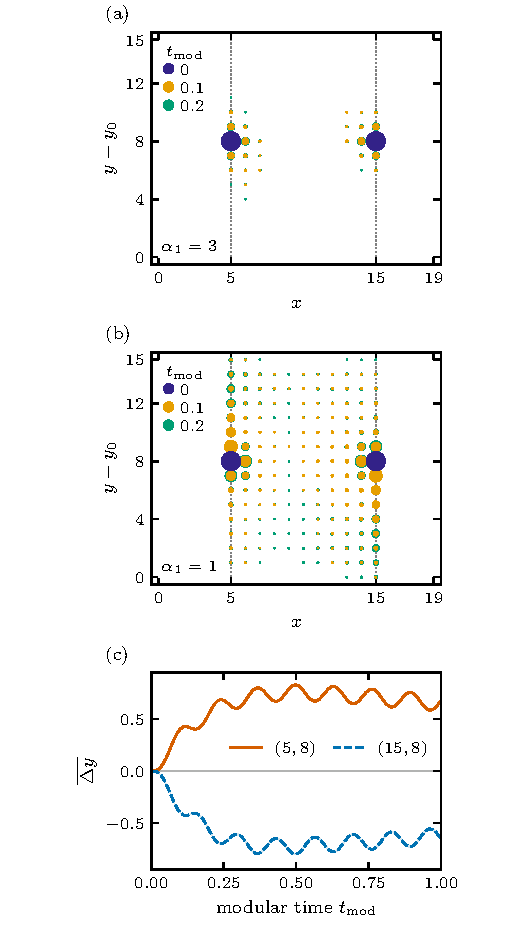
\includegraphics[width=\columnwidth]{Figure_10_modular_evolution.pdf}
    \caption{\newtext{\textbf{Modular evolution on the walls.} Two incoherent orbital profiles are initialized at each source cell $(x,\delta y)=(5,8)$ or $(15,8)$ in a half-cylinder of 16 rows. The states come from $S=100$ independent random-pure trajectories per $\alpha_1=1,3$ on a $20\times32$ lattice after 64 cycles. (a,b) Mean densities at $t_{\rm mod}=0,0.1,0.2$ (purple, orange, green) for (a) $\alpha_1=3$ and (b) $\alpha_1=1$. (c) Mean center-of-mass displacement $\overline{\Delta y_{x_s}}$ from the initial row $\delta y=8$, defined in Eq.~\eqref{eq:ModularDisplacement}, for $\alpha_1=1$. Solid and dashed lines denote $x_s=5$ and $15$; each five-column window is normalized by its retained weight before averaging. Each observable is evaluated per cut, then averaged over 32 origins and trajectories. Bands are one trajectory SEM. Centered occupations are clipped at $\pm(1-10^{-10})$ when constructing $h_A$.}}
    \label{fig:Modular}
\end{figure}

{\color{blue}
\subsection{Trajectory-averaged dynamics}
\label{sec:TrajectoryAveraged}

Finally, we ask what remains of the boundary criticality when the measurement record is discarded. Averaging an elementary step gives $\mc E_{j,s}(\hat\rho)=\sum_{\mathrm m}\hat K_j(\mathrm m)\hat\rho\hat K_j^\dagger(\mathrm m)$. It can be written exactly as $\mc E_{i,\sigma}=\mathrm{Id}+\mc L_{i,\sigma}$, with
\begin{align}
 \mc L_{i,-}&=\mc D[\hat\chi_{i,-}^\dagger]+\mc D[\hat{\mc N}_{i,-}],\nonumber\\
 \mc L_{i,+}&=\mc D[\hat\chi_{i,+}]+\mc D[\hat{\mc N}_{i,+}],
 \label{eq:AveragedChannel}
\end{align}
where $\mc D[\hat L]\hat\rho=\hat L\hat\rho\hat L^\dagger-\tfrac12\{\hat L^\dagger\hat L,\hat\rho\}$. This is an identity for the discrete reset, not a short-time approximation; the dephasing term belongs to the same measurement-and-feedback step. The two-point function closes, with \claudeadd{$P_j=W_jW_j^\dagger$}, $Q_j=\Id-P_j$, and target occupation $s_j=s_\sigma$ for the mode reset at step $j$,
\begin{equation}
 \overline G'=Q_j\overline GQ_j+s_jP_j.
 \label{eq:AveragedUpdate}
\end{equation}
In fact, the exact reset preserves Gaussianity for Gaussian input: in a basis beginning with the measured mode, it replaces that mode by its target state and retains the reduced state on the orthogonal modes. Equation~\eqref{eq:AveragedUpdate} holds even for non-Gaussian inputs. We can therefore compute the averaged two-point dynamics without sampling trajectories.

Figure~\ref{fig:TrajectoryAveraged}(a) shows the occupation spectrum after 128 cycles at $N_y=64$, starting from maximal mixing. At $\alpha_1=1$, branches connect the nearly filled and empty bands, whereas the trivial control has no analogous crossing. Such mean-state boundary structure can also arise in dissipative Chern preparation~\cite{Goldstein2019}. However, the squared two-point function formed from $\overline G$, namely $C_{\overline G}^{\rm av}$, is short ranged for both parameters [Fig.~\ref{fig:TrajectoryAveraged}(b)]. It differs from the trajectory-resolved $\overline{C_G^{\rm av}}$ in Fig.~\ref{fig:Correlations}.

}

\begin{figure}[!htbp]
    \centering
    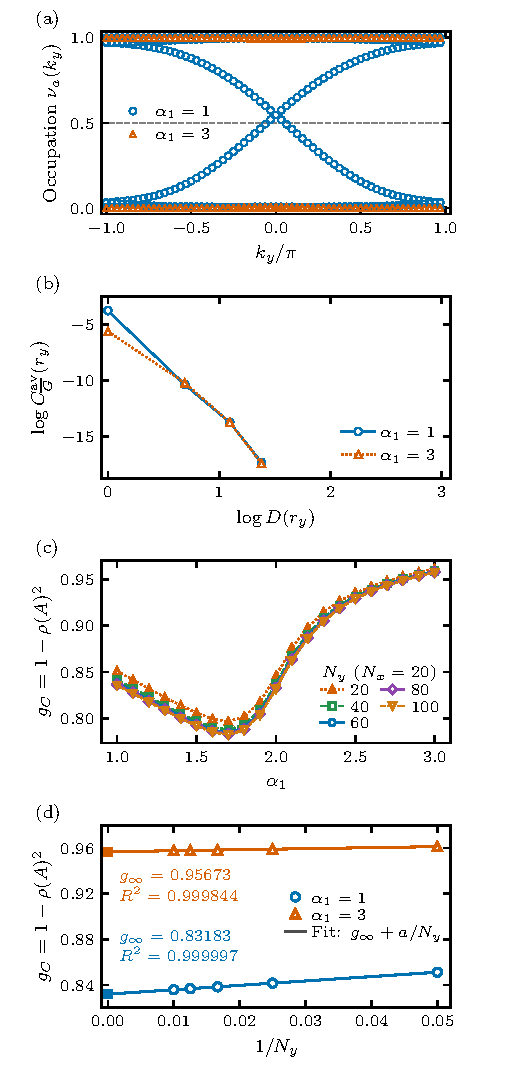
\includegraphics[width=\columnwidth]{Figure_11_mean_channel.pdf}
    \caption{\newtext{\textbf{Trajectory-averaged dynamics and channel gap.} (a) Occupations of the translation-averaged two-point matrix and (b) its squared correlation at $N_y=64$, after 128 cycles from maximal mixing, for $\alpha_1=1,3$. Correlations below $10^{-8}$ are not displayed. (c) Exact multiplier gap $g_C=1-\rho(A)^2$ versus $\alpha_1$ at fixed $N_x=20$ and $N_y=20,40,60,80,100$. (d) Fits $g_\infty+a/N_y$ at $\alpha_1=1,3$, using all five sizes; squares at $1/N_y=0$ mark extrapolated intercepts. Outcomes are averaged analytically in the fixed repeated raster schedule, so there is no sampled-trajectory count or SEM. \claudedel{The gap is dimensionless.}}}
    \label{fig:TrajectoryAveraged}
\end{figure}

{\color{blue}
We further quantify relaxation of the averaged channel. For one fixed raster cycle of $M$ elementary resets,
\begin{equation}
 \overline G_{n+1}=A\overline G_nA^\dagger+B,\qquad A=Q_M\cdots Q_1,
 \label{eq:CycleChannel}
\end{equation}
where $B$ is independent of the incoming state. Deviations from stationarity propagate as $A\delta G A^\dagger$, so the dimensionless covariance gap is
\begin{equation}
 g_C=1-\rho(A)^2,
 \label{eq:ChannelGap}
\end{equation}
with $\rho(A)$ the spectral radius. For these exact resets, higher charge-neutral correlations cannot decay more slowly than the two-point function. Consequently $g_C$ is also the many-body channel gap in the charge-neutral and parity-even sectors, as shown in Appendix~\ref{app:ChannelGap}. Charge neutrality means $[\hat\rho,\hat Q]=0$, where $\hat Q=\sum_i\hat c_i^\dagger\hat c_i$ is the physical charge; it does not require particle number to remain fixed along a trajectory. \claudedel{The corresponding exponential rate is $-2\log\rho(A)$ per cycle, distinct from both $g_C$ and the trajectory-purification gap of Eq.~\eqref{eq:LyapunovFromOccupations}.}\claudeadd{Equivalently, deviations decay at the rate $-2\log\rho(A)$ per cycle. This rate characterizes the averaged channel and should not be confused with the trajectory Lyapunov gap of Eq.~\eqref{eq:LyapunovFromOccupations}.}

Figure~\ref{fig:TrajectoryAveraged}(c) shows that $g_C$ remains nonzero across $1\leq\alpha_1\leq3$ for $N_y=20,40,60,80,100$ at fixed $N_x=20$. Fitting $g_C=g_\infty+a/N_y$ gives $g_\infty\approx0.83$ and $0.96$ for $\alpha_1=1$ and $3$, respectively [Fig.~\ref{fig:TrajectoryAveraged}(d)]. These are finite-width extrapolations of the channel spectrum, not purification rates or bounds on a size-uniform mixing time.

\claudeadd{The intermediate occupations in Fig.~\ref{fig:TrajectoryAveraged}(a) do not signal slow averaged dynamics. In Eq.~\eqref{eq:CycleChannel}, the relaxation is controlled by $A$ alone, whereas the stationary two-point function also depends on the source $B$, which carries the target occupations. An occupation near $1/2$ thus reflects a mixture over records, in which different trajectories occupy the wall modes differently, rather than a slow mode of the channel. Balanced single-mode gain and loss, $\mc L=\eta(\mc D[\hat c]+\mc D[\hat c^\dagger])$, relaxes in the same way at the finite rate $\eta$ to the maximally mixed occupation $n=1/2$. A similar separation between purity and damping gaps appears in dissipatively prepared topological states~\cite{BardynEtAl2013}.}

The contrast is therefore between the critical conditioned states and their outcome average. The algebraic correlations and logarithmic entanglement established above require access to individual records; discarding them gives short-range two-point correlations and a channel with a finite relaxation gap over the sizes studied. In this sense, the boundary criticality lives at the level of the trajectories. \claudedel{To our knowledge, preparation of such critical chiral boundaries by repeated finite-range measurements and local feedback under Born sampling has not previously been demonstrated.} \claudedel{This comparison concerns monitored adaptive preparation, rather than unitary or unmonitored dissipative preparation.} \claudecom{Removed here; the novelty claim and the comparison with unitary and dissipative preparation now live in the introduction.}
}



\FloatBarrier
{\color{blue}\section{Conclusions and Outlook}
\label{sec:Conclusions}}

\GPT{Suggested points: summarize the distinction between trajectory-resolved critical chiral boundaries and the short-range outcome average; separate the evidence for criticality and chirality from the open identification with an equilibrium ground state.}

\claudeadd{We have shown that repeated finite-range occupation measurements with purely local feedback prepare chiral critical boundaries without postselection. In a slab geometry, the circuit prepares a Chern bulk, and each measurement record yields a pure state whose interfaces carry algebraic correlations, logarithmic entanglement and charge fluctuations with coefficients close to those of a free chiral fermion, half a unit of entropy coefficient per wall, and opposite modular handedness on the two walls. The same walls host the slowest modes of the purification dynamics. All of these signatures are properties of the record-resolved ensemble. Discarding the record leaves a mixed state with short-range correlations and a gapped averaged channel, consistent with the obstructions to dissipative preparation of Chern insulators. Whether the conditioned wall states are equivalent to the ground state of an equilibrium chiral Luttinger liquid remains open.}

\claudeadd{Because the trajectory-level criticality is invisible in the averaged state, observing it experimentally faces the postselection problem of monitored dynamics. Here, the Gaussian structure helps: each record's state can be computed classically from the measured outcomes, which enables postselection-free estimators that combine single-copy measurements with classical simulation~\cite{GarrattAltman2024,McGinley2024}.}
\claudecom{On the outlook items: (i) observability, as in the paragraph above; (ii) depth: whether a layered schedule of commuting measurements, started from a product state, reaches the critical walls in a number of cycles independent of $N_y$, given that the Lyapunov gap suggests relaxation times growing with $N_y$; (iii) class D and vortices with Majorana zero modes, as GPT suggests, which would need a different stabilizer construction; (iv) robustness to imperfect feedback or interactions. Pick two; four is too many for an outlook.}

\GPT{Possible extensions include other symmetry classes and programmable point defects, such as vortices hosting Majorana zero modes in two-dimensional superconducting systems. This is an outlook direction, not a result established here.}


{\color{blue}
\begin{acknowledgments}
We used OpenAI Codex and Anthropic Claude to assist with manuscript drafting and editing, plotting code and figure preparation, and the exploration of analytical arguments. The authors take responsibility for the final content, including the scientific analysis, conclusions, and references.
\end{acknowledgments}
}

\FloatBarrier
\appendix
\setcounter{figure}{0}
\renewcommand{\thefigure}{A\arabic{figure}}
\renewcommand{\theHfigure}{A\arabic{figure}}

{\color{blue}\section{Finite-Range Truncation}
\label{app:Truncation}}

{\color{blue}
In this Appendix, we examine how the finite window in Eq.~\eqref{eq:TruncatedOW} changes the OW frame. We distinguish the persistence of the form-factor obstruction from the band mixing and critical-point shift caused by truncation. \claudeadd{We then show that the parent Hamiltonian built from the truncated modes provably remains in the target phase whenever the truncation error is smaller than one half, a condition satisfied already for $w=1$.} The dynamical bulk validation is given separately in Sec.~\ref{sec:BulkTopology}.
}

\subsection{Momentum-space obstruction}

Let $P_\pm(\bk)=|u_\pm(\bk)\rangle\langle u_\pm(\bk)|$ in a local gauge. The form factor associated with the trial orbital $\tau_\nu$ is
\begin{equation}
    f_{\nu,\pm}(\bk)\propto\langle u_\pm(\bk)|\tau_\nu\rangle,
    \qquad
    P_\pm(\bk)|\tau_\nu\rangle\propto f_{\nu,\pm}(\bk)|u_\pm(\bk)\rangle,
    \label{eq:FormFactor}
\end{equation}
normalized over the Brillouin zone. For a band with nonzero Chern number, the form factor cannot be smooth and nonzero everywhere~\cite{BhuiyanPanJian2026}. Its isolated zeros carry phase windings $\omega_a=(2\pi)^{-1}\oint_{\partial D_a}d\bk\cdot\nabla_{\bk}\arg f_{\nu,\pm}$ around counterclockwise loops $\partial D_a$, which satisfy
\begin{equation}
    \sum_a\omega_a=-\mc C_\pm.
    \label{eq:ZeroWinding}
\end{equation}
At $\alpha=1$, the lower-band $A$-family form factor has a single zero at $\bk/\pi=(1/2,0)$ with winding $-1$.

The truncation window multiplies the OW function in real space and therefore convolves it in momentum space. Writing $\widetilde g_w(\bs q)$ for the Fourier transform of the centered window, the Bloch transform of a truncated OW mode and its effective form factor are
\begin{align}
    |\phi_{\nu,\pm;w}(\bk')\rangle&\propto\int_{\mr{BZ}}\frac{d^2\bk}{(2\pi)^2}\,\widetilde g_w(\bk'-\bk)\,f_{\nu,\pm}(\bk)\,|u_\pm(\bk)\rangle,\nonumber\\
    f^{\rm eff}_{\nu,\pm;w}(\bk')&\propto\langle u_\pm(\bk')|\phi_{\nu,\pm;w}(\bk')\rangle.
    \label{eq:EffectiveFormFactor}
\end{align}
Since $|\phi_{\nu,\pm;w}(\bk)\rangle$ is a finite Fourier sum, it is smooth and periodic. The in-band component $P_\pm|\phi_{\nu,\pm;w}\rangle\propto f^{\rm eff}_{\nu,\pm;w}|u_\pm\rangle$ thus plays the same role as $P_\pm|\tau_\nu\rangle$, with the constant trial orbital replaced by a smooth momentum-dependent one. Hence, the zeros of $f^{\rm eff}_{\nu,\pm;w}$ also obey Eq.~\eqref{eq:ZeroWinding}. A finite window may move, split, or recombine the zeros, but it cannot remove them while $\mc C_\pm\neq0$.

Figure~\ref{fig:Truncation}(a,b) confirms this for the lower-band $A$-family mode at $\alpha=1$. The zero stays on the line $k_y=0$ and carries winding $-1$ for every $w=1,\ldots,12$. It sits at $k_x/\pi\approx0.492$ for $w=1$ and rapidly approaches the untruncated position $k_x/\pi=1/2$ as $w$ increases.

\begin{figure}[!htbp]
    \centering
    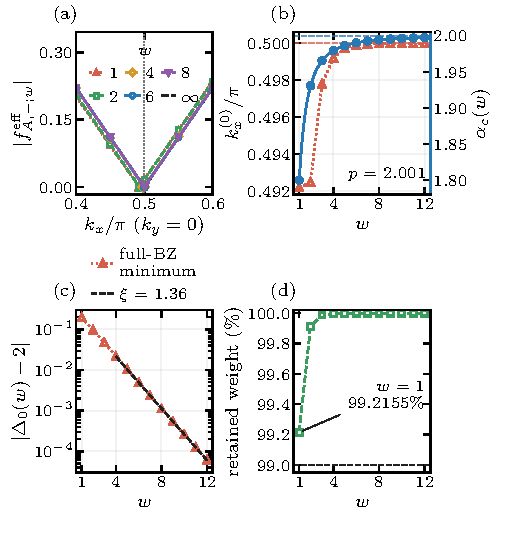
\includegraphics[width=\columnwidth]{Figure_A01_ow_truncation.pdf}
    \caption{\textbf{Truncated OW modes at $\alpha=1$.} (a) Effective form factor $|f^{\rm eff}_{A,-;w}|$ along $k_y=0$ for $w=1,2,4,6,8,\infty$. Symbols mark the zeros, and the dotted line marks the untruncated zero. (b) Position of the winding-$(-1)$ zero (red, left axis) and the critical parameter $\alpha_c(w)$ of the truncated parent Hamiltonian (blue, right axis) with the fit of Eq.~\eqref{eq:CriticalDrift}. Dashed lines mark the $w=\infty$ values. (c) Deviation of the half-filling gap $\Delta_0(w)$ of the truncated parent Hamiltonian from its untruncated value, with an exponential fit for $w\geq4$. (d) Fraction of the squared OW norm retained inside the window.}
    \label{fig:Truncation}
\end{figure}

\subsection{Band mixing and frustration}

The effective form factor is only the in-band part of the truncated mode. Because $\langle u_\mp(\bk')|u_\pm(\bk)\rangle\neq0$ for $\bk\neq\bk'$, the convolution in Eq.~\eqref{eq:EffectiveFormFactor} also generates a component in the opposite band, which vanishes only in the untruncated limit, where $\widetilde g_w$ becomes a delta function. At $\alpha=1$, the weight of a truncated mode in the opposite band,
\begin{equation}
    \epsilon_w=\int_{\mr{BZ}}\frac{d^2\bk}{(2\pi)^2}\,\big|\langle u_\mp(\bk)|\phi_{\nu,\pm;w}(\bk)\rangle\big|^2,
    \label{eq:BandLeakage}
\end{equation}
is $\epsilon_1\approx4\times10^{-3}$, $\epsilon_2\approx4\times10^{-4}$, and $\epsilon_4\approx1\times10^{-5}$, identical for all four choices of $\nu$ and $\pm$. At $w=1$, this is about half of the $0.8\%$ of squared weight discarded by the window [Fig.~\ref{fig:Truncation}(d)].

This band mixing lifts the linear dependence among the OW modes. On an $8\times8$ periodic lattice at $\alpha=1$, the 128 untruncated lower-band OW modes span exactly the 64-dimensional lower band. For $w=1$ and $w=2$, the 128 truncated lower-band modes instead span the entire 128-dimensional single-particle space, as do the truncated upper-band modes. Filling every truncated lower-band mode would then fill every single-particle state, which is incompatible with emptying any truncated upper-band mode. Hence, no many-body state satisfies all truncated stabilizing conditions. The smallest singular value of the matrix whose rows are the truncated lower-band modes is about $10^{-3}$ at $w=1$, so the modes are only weakly independent and the frustration is correspondingly weak.

\subsection{Truncated parent Hamiltonian}
\label{app:TruncatedParent}

To determine whether the truncated modes still describe the target phase, we construct the translation-invariant single-particle parent Hamiltonian generated by the truncated OW frame,
\begin{align}
    h_w(\bk)=\sum_{\nu=A,B}\Big[&|\phi_{\nu,+;w}(\bk)\rangle\langle\phi_{\nu,+;w}(\bk)|\nonumber\\
    &-|\phi_{\nu,-;w}(\bk)\rangle\langle\phi_{\nu,-;w}(\bk)|\Big],
    \label{eq:TruncatedParent}
\end{align}
which is traceless. If every truncated mode remained in its band, $h_w(\bk)=a(\bk)P_+(\bk)-b(\bk)P_-(\bk)$ with $a,b\geq0$, and its occupied band would coincide with the target lower band wherever $h_w$ is gapped. Band mixing is what can change its topology.

{\color{orange}
For the square window and the $\sigma^x$ trial orbitals, $h_w$ takes a simple form. Let $P_-(\boldsymbol d)=\int_{\mr{BZ}}\frac{d^2\bk}{(2\pi)^2}e^{\ii\bk\cdot\boldsymbol d}P_-(\bk)$ be the real-space kernel of the target projector, and define its windowed Fourier series
\begin{equation}
    F_w(\bk)=\sum_{|d_x|,|d_y|\leq w}P_-(\boldsymbol d)\,e^{-\ii\bk\cdot\boldsymbol d}.
    \label{eq:WindowedProjector}
\end{equation}
Since the kernel is Hermitian, $P_-(\boldsymbol d)^\dagger=P_-(-\boldsymbol d)$, and the window is inversion symmetric, $F_w$ is Hermitian. Multiplying the centered OW function by the window and Fourier transforming gives the Bloch transforms
\begin{equation}
    |\phi_{\nu,-;w}\rangle=\frac{F_w|\tau_\nu\rangle}{\sqrt{Z_w}},
    \qquad
    |\phi_{\nu,+;w}\rangle=\frac{(\Id-F_w)|\tau_\nu\rangle}{\sqrt{Z_w}},
    \label{eq:TruncatedBloch}
\end{equation}
where we used $P_+=\Id-P_-$ and the fact that the window contains the origin. The normalization $Z_w$ is the same for all four modes. To see this, write $F_w=\frac12(\Id-\boldsymbol d_w\cdot\boldsymbol\sigma)$. The Brillouin-zone average of $d_{w,x}$ vanishes by reflection symmetry, and $\tau_A$ and $\tau_B$ have vanishing expectation values of $\sigma^y$ and $\sigma^z$. Hence $Z_w=\int_{\mr{BZ}}\frac{d^2\bk}{(2\pi)^2}\langle\tau_\nu|F_w^2|\tau_\nu\rangle=\frac14(1+\langle|\boldsymbol d_w|^2\rangle_{\mr{BZ}})$ for both $\nu$, and the same holds for $\Id-F_w$. Substituting Eq.~\eqref{eq:TruncatedBloch} into Eq.~\eqref{eq:TruncatedParent} and using $\sum_\nu|\tau_\nu\rangle\langle\tau_\nu|=\Id$, the quadratic terms cancel, and
\begin{equation}
    h_w(\bk)=\frac{\Id-2F_w(\bk)}{Z_w}.
    \label{eq:FrameIdentity}
\end{equation}
The occupied band of $h_w$ is therefore the spectral subspace of $F_w$ with eigenvalue above $1/2$. We denote its projector by $R_w(\bk)$.

Equation~\eqref{eq:FrameIdentity} makes the topology of $h_w$ transparent, since $F_w$ is a truncation of $P_-$. Consider the straight path $F_s=P_-+s(F_w-P_-)$ with $s\in[0,1]$, and let
\begin{equation}
    \delta_w=\sup_{\bk}\big\|F_w(\bk)-P_-(\bk)\big\|_{\rm op}.
    \label{eq:TruncationError}
\end{equation}
Along the path, the eigenvalues of $F_s$ stay within $s\delta_w$ of 0 and 1. If $\delta_w<1/2$, none of them crosses $1/2$, so the spectral projector of $F_s$ above $1/2$ deforms smoothly at fixed rank from $P_-$ to $R_w$. Since an integer cannot change continuously~\cite{AvronSeilerSimon1983}, the occupied band of $h_w$ then carries the target Chern number, and its gap obeys $\min_{\bk,n}|E_n[h_w(\bk)]|\geq(1-2\delta_w)/Z_w$. By the triangle inequality, $\delta_w$ is bounded by the discarded tail of the kernel,
\begin{equation}
    \delta_w\leq\sum_{\boldsymbol d\notin\text{window}}\big\|P_-(\boldsymbol d)\big\|_{\rm op},
    \label{eq:TailBound}
\end{equation}
which decays exponentially with $w$ inside the gapped phase. At $\alpha=1$, the tail sum is about $0.46$ already for $w=1$, so the condition $\delta_1<1/2$ is guaranteed without sampling momenta. Evaluating Eq.~\eqref{eq:TruncationError} directly gives $\delta_1\approx0.10$ and $Z_1\approx0.496$, so the bound $(1-2\delta_1)/Z_1\approx1.62$ is consistent with the gap $\Delta_0(1)\approx1.80$ found below. Equivalently, the overlap $\operatorname{tr}[P_-(\bk)R_1(\bk)]$ stays above $0.99$ throughout the Brillouin zone, so the occupied band of $h_1$ never becomes orthogonal to the target band.

Note that $h_w$ is finite range, gapped, and carries Chern number 1. This does not contradict the no-go theorem of Ref.~\cite{DubailRead2015}, which concerns compactly supported functions that span a Chern band. The projector $R_w$ is obtained from $F_w$ by a spectral projection, which restores exponential tails, so $R_w$ is not spanned by compactly supported functions.
}

At $\alpha=1$, the half-filling gap $\Delta_0(w)=\min_{\bk,n}|E_n[h_w(\bk)]|$ rapidly approaches its untruncated value $\Delta_0(\infty)=2$ [Fig.~\ref{fig:Truncation}(c)]. Already at $w=1$, the parent is well gapped, with $\Delta_0(1)\approx1.80$, and its occupied band carries Chern number 1, equal to that of the target band. In contrast, the onsite limit $w=0$ gives a momentum-independent $h_0$ with a trivial occupied band. \claudeadd{There, $\|F_0-P_-\|_{\rm op}\approx0.75$ at the $\Gamma$ point, so the condition $\delta_0<1/2$ fails, and the straight path closes its gap.} Thus, $w=1$ suffices to keep the truncated parent in the target phase, which is why we use $w=1$ in the main text.

As $\alpha$ increases, the gap of $h_w$ closes at the $\Gamma$ point at a $w$-dependent value $\alpha_c(w)<2$ [Fig.~\ref{fig:Truncation}(b)], with $\alpha_c(1)\approx1.80$, $\alpha_c(2)\approx1.93$, and $\alpha_c(4)\approx1.98$. \claudeadd{By Eq.~\eqref{eq:FrameIdentity}, the gap closes where an eigenvalue of $F_w$ crosses $1/2$. At $\Gamma$, reflection symmetry removes the $\sigma^x$ and $\sigma^y$ components, so $F_w(\Gamma)=\frac12[\Id-d_{w,z}(\Gamma)\sigma^z]$, and $\alpha_c(w)$ is simply the root of the single function $d_{w,z}(\Gamma)$ of $\alpha$.} For $w\geq3$, the drift is well described by
\begin{equation}
    2-\alpha_c(w)\simeq\frac{0.40}{(w+0.42)^2},
    \label{eq:CriticalDrift}
\end{equation}
which extrapolates to the untruncated transition $\alpha_c(\infty)=2$. For $\alpha_c(w)<\alpha<2$, the occupied band of $h_w$ is trivial while the target band has $\mc C=1$. For instance, at $\alpha=1.9$, the occupied band of $h_w$ has Chern number 0 for $w=1$ and 1 for $w=4$. This shift is a direct consequence of band mixing\claudeadd{, through the growth of $\delta_w$ as the kernel $P_-(\boldsymbol d)$ becomes longer ranged near the target transition}.

\claudeadd{We emphasize that these statements concern the auxiliary band of $h_w$, not the conditioned states of the circuit. They provide supporting evidence that finite-range truncation does not change the target phase, while the topology of the prepared states is established directly by the real-space Chern number in Sec.~\ref{sec:BulkTopology}.}

{\color{blue}
The shift in Fig.~\ref{fig:Truncation} concerns the translation-invariant parent built from the truncated modes, rather than a change of the original QWZ target transition. The mutual-information crossover in Fig.~\ref{fig:MutualInformation}(b) lies in the same parameter region, but its finite-width peak does not independently determine a dynamical critical point.
}

\FloatBarrier
\section{Ancilla Elimination and Fermion Counting}
\label{app:FermionCounting}

In this Appendix, we derive the gain and loss operations of Eq.~\eqref{eq:GainLoss}, their $U(1)$ symmetry, and their relation to fermion counting. We write $\hat\chi$ for a single normalized truncated OW mode, $\hat{\mc N}=\hat\chi^\dagger\hat\chi$, and $\hat d$ for a fresh ancillary mode, which anticommutes with $\hat\chi$ and $\hat\chi^\dagger$.

\subsection{Gain and loss from the fSWAP gate}

\newtext{The gate exchanging the physical mode $\hat\chi$ and the ancillary mode $\hat d$ is~\cite{BhuiyanPanJian2026}}
\begin{align}
    \fSWAP(\hat\chi,\hat d)
    &=\exp\!\left[\ii\frac{\pi}{2}(\hat\chi^\dagger-\hat d^\dagger)(\hat\chi-\hat d)\right]\nonumber\\
    &=\hat\Id-\hat{\mc N}-\hat n_a+\hat\chi^\dagger\hat d+\hat d^\dagger\hat\chi,
    \label{eq:fSWAP}
\end{align}
\newtext{where $\hat n_a=\hat d^\dagger\hat d$. We order ancillary creation operators to the left of physical creation operators, as in the matrix elements of Eq.~\eqref{eq:GainLoss}.}

For gain, let $\newtext{\kett{\psi_0}}=(\hat\Id-\hat{\mc N})\newtext{\kett{\psi}}$ for an arbitrary physical state $\newtext{\kett{\psi}}$, so that $\hat\chi\newtext{\kett{\psi_0}}=0$. With the ancilla operator ordered to the left, the fresh occupied ancilla gives the composite state $\hat d^\dagger\newtext{\kett{\psi_0}}$. Acting with the three parts of Eq.~\eqref{eq:fSWAP} and using $\hat n_a\hat d^\dagger\newtext{\kett{\psi_0}}=\hat d^\dagger\newtext{\kett{\psi_0}}$, we find
\begin{align}
    (\hat\Id-\hat{\mc N}-\hat n_a)\,\hat d^\dagger\newtext{\kett{\psi_0}}&=-\hat d^\dagger\hat{\mc N}\newtext{\kett{\psi_0}}=0,\nonumber\\
    \hat\chi^\dagger\hat d\,\hat d^\dagger\newtext{\kett{\psi_0}}&=\hat\chi^\dagger(\hat\Id-\hat d^\dagger\hat d)\newtext{\kett{\psi_0}}=\hat\chi^\dagger\newtext{\kett{\psi_0}},\nonumber\\
    \hat d^\dagger\hat\chi\,\hat d^\dagger\newtext{\kett{\psi_0}}&=-(\hat d^\dagger)^2\hat\chi\newtext{\kett{\psi_0}}=0.
    \label{eq:GainSteps}
\end{align}
Hence, $\fSWAP\,\hat d^\dagger\newtext{\kett{\psi_0}}=\hat\chi^\dagger\newtext{\kett{\psi_0}}$ with the ancilla left empty. Projecting onto the empty ancilla gives $\hat\chi^\dagger(\hat\Id-\hat{\mc N})\newtext{\kett{\psi}}=\hat\chi^\dagger\newtext{\kett{\psi}}$, since $\hat\chi^\dagger\hat{\mc N}=(\hat\chi^\dagger)^2\hat\chi=0$. This is the first line of Eq.~\eqref{eq:GainLoss}.

For loss, let $\newtext{\kett{\psi_1}}=\hat{\mc N}\newtext{\kett{\psi}}$ with the ancilla empty. Then $(\hat\Id-\hat{\mc N}-\hat n_a)\newtext{\kett{\psi_1}}=0$ and $\hat\chi^\dagger\hat d\newtext{\kett{\psi_1}}=0$, so $\fSWAP\,\newtext{\kett{\psi_1}}=\hat d^\dagger\hat\chi\newtext{\kett{\psi_1}}$ with the ancilla left occupied. Removing the occupied ancilla gives $\hat\chi\hat{\mc N}\newtext{\kett{\psi}}=\hat\chi\newtext{\kett{\psi}}$, since $\hat\chi\hat{\mc N}=(\hat\Id-\hat\chi^\dagger\hat\chi)\hat\chi=\hat\chi$. This is the second line of Eq.~\eqref{eq:GainLoss}. In both cases, the final ancilla state is fixed by the measurement outcome, so the composite state is a product state, and discarding the ancilla leaves exactly these operators.

\subsection{Weak \texorpdfstring{$U(1)$}{U(1)} symmetry}

Let $\hat Q=\sum_{\bfr,\mu}\hat c^\dagger_{\bfr,\mu}\hat c_{\bfr,\mu}$ be the physical charge. Since $\hat\chi^\dagger$ is a linear combination of the $\hat c^\dagger_{\bfr,\mu}$, we have $e^{\ii\theta\hat Q}\hat\chi^\dagger e^{-\ii\theta\hat Q}=e^{\ii\theta}\hat\chi^\dagger$. Each Kraus operator in Eqs.~\eqref{eq:KrausLower} and \eqref{eq:KrausUpper} therefore carries a definite charge $q(\mathrm{m})$,
\begin{equation}
    e^{\ii\theta\hat Q}\hat K(\mathrm{m})e^{-\ii\theta\hat Q}=e^{\ii\theta q(\mathrm{m})}\hat K(\mathrm{m}),
    \label{eq:KrausCharge}
\end{equation}
with $q\in\{0,+1\}$ for the lower band and $q\in\{0,-1\}$ for the upper band. The phases cancel between $\hat K$ and $\hat K^\dagger$ in the averaged channel, so
\begin{equation}
    \mc E\big(e^{\ii\theta\hat Q}\hat\rho\,e^{-\ii\theta\hat Q}\big)=e^{\ii\theta\hat Q}\,\mc E(\hat\rho)\,e^{-\ii\theta\hat Q}.
    \label{eq:WeakU1}
\end{equation}
This is a weak $U(1)$ symmetry~\cite{BucaProsen2012,AlbertJiang2014}. It is not a strong symmetry, since the gain and loss operators do not commute with $\hat Q$. In the composite system, by contrast, both the occupation measurement and the fSWAP gate commute with $\hat Q+\hat n_a$.

\subsection{Fermion counting run to completion}

Consider continuous, perfectly efficient monitoring of gain into the mode $\hat\chi$ at rate $\gamma$, i.e., quantum jumps generated by $\sqrt\gamma\,\hat\chi^\dagger$ with every jump recorded~\cite{StarchlFischerSieberer2025}. Since $\hat\chi\hat\chi^\dagger=\hat\Id-\hat{\mc N}$ is a projector, the evolution without a click over a time $t$ is
\begin{equation}
    \hat M_0(t)=e^{-\gamma t\,\hat\chi\hat\chi^\dagger/2}=\hat{\mc N}+e^{-\gamma t/2}(\hat\Id-\hat{\mc N}).
    \label{eq:NoClick}
\end{equation}
A click at time $t'\in(0,t)$ gives
\begin{equation}
    \hat M(t')=e^{-\gamma(t-t')\hat\chi\hat\chi^\dagger/2}\sqrt\gamma\,\hat\chi^\dagger e^{-\gamma t'\hat\chi\hat\chi^\dagger/2}=\sqrt\gamma\,e^{-\gamma t'/2}\,\hat\chi^\dagger,
    \label{eq:Click}
\end{equation}
where we used $\hat\chi^\dagger\hat{\mc N}=0$ and $(\hat\Id-\hat{\mc N})\hat\chi^\dagger=0$. A second click is impossible, since $(\hat\chi^\dagger)^2=0$. These operators are complete,
\begin{align}
    &\hat M_0^\dagger(t)\hat M_0(t)+\int_0^tdt'\,\hat M^\dagger(t')\hat M(t')\nonumber\\
    &\qquad=\hat{\mc N}+e^{-\gamma t}(\hat\Id-\hat{\mc N})+(1-e^{-\gamma t})(\hat\Id-\hat{\mc N})=\hat\Id.
    \label{eq:CountingCompleteness}
\end{align}
For $\gamma t\gg1$, $\hat M_0(t)\to\hat{\mc N}$, and every click branch leaves the same normalized state $\hat\chi^\dagger\kett{\psi}/\|\hat\chi^\dagger\kett{\psi}\|$, independent of the click time. Recording only whether a click occurred therefore reproduces the lower-band Kraus operators of Eq.~\eqref{eq:KrausLower}, with $\mathrm{m}=1$ corresponding to no click and $\mathrm{m}=0$ to a click. Monitoring loss with jumps $\sqrt\gamma\,\hat\chi$ reproduces Eq.~\eqref{eq:KrausUpper} in the same way. At finite $\gamma t$, the no-click branch retains the component $e^{-\gamma t/2}(\hat\Id-\hat{\mc N})$, and the correction is incomplete.

{\color{blue}
\section{Supporting Entanglement Diagnostics}
\label{app:MutualInformation}

The entropy contour provides a spatial complement to the strip scaling in Sec.~\ref{sec:Entanglement}. For each translated half-strip we evaluate $s_1(x,\delta y)$ from Eq.~\eqref{eq:Contour}, align the rows by $\delta y=y-y_0$, and average first over all origins and then over trajectories. At $\alpha_1=1$, the contour has weight along the physical walls as well as along the entanglement cuts [Fig.~\ref{fig:MutualInformation}(a)]. For $\alpha_1=3$, the dominant weight remains near the cuts. This distinction separates boundary entanglement from an area-law contribution that can persist in the trivial control.

We also consider two antipodal full-width strips $a,b$, each of width $\ell=N_y/4$, and compute
\begin{equation}
 I_{a,b}=S(a)+S(b)-S(a\cup b).
 \label{eq:MutualInformation}
\end{equation}
The subtraction is performed for each trajectory and translation before either average. For a free Dirac fermion, the two-interval result on a circle gives~\cite{CasiniHuerta2009,CalabreseCardyTonni2009}
\begin{equation}
 I^{\rm Dirac}_{a,b}=-\frac{c}{3}\log(1-x),\qquad
 x=\sin^2\!\left(\frac{\pi\ell}{N_y}\right).
 \label{eq:DiracMI}
\end{equation}
With $c=1$ and $\ell=N_y/4$, this yields $(\log2)/3$, independent of circumference. \claudedel{We use it as an equilibrium comparison, without assuming that the adaptive circuit prepares that ground state.}\claudeadd{We use it as a reference value for a free Dirac fermion formed by the two counterpropagating walls.}

At $\alpha_1=1$, the mean mutual information moves toward this value as $N_y$ increases [Fig.~\ref{fig:MutualInformation}(b)]. It develops a finite-size peak near $\alpha_1\simeq1.7$ and becomes small by $\alpha_1\gtrsim2$. The peak lies near the shifted truncated-parent transition $\alpha_c(1)\simeq1.8$ in Fig.~\ref{fig:Truncation}; bulk correlations and the finite slab width also contribute in this regime. Hence the figure supports the disappearance of the wall signal upon entering the trivial regime, rather than fixing a precise dynamical critical point. The parameter still jumps at the interfaces for $\alpha_1=3$, so an interface mismatch alone does not account for the critical wall correlations.
}

\begin{figure}[!htbp]
    \centering
    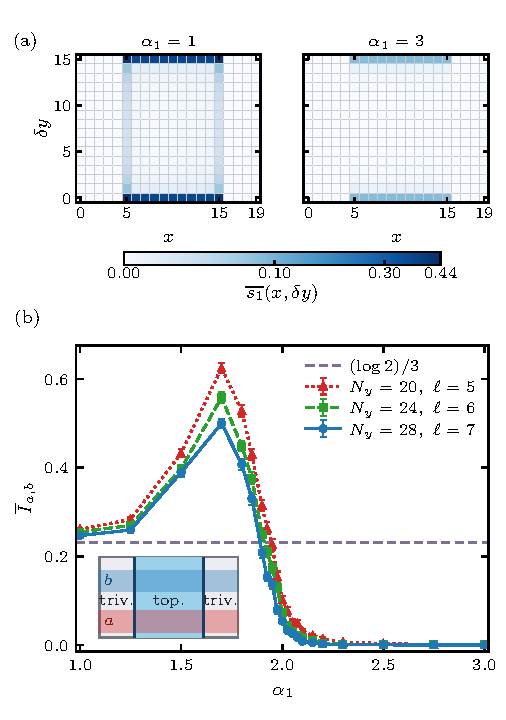
\includegraphics[width=\columnwidth]{Figure_A02_mutual_information.pdf}
    \caption{\newtext{\textbf{Spatial entanglement and antipodal mutual information.} (a) Mean entropy contours for $\alpha_1=1,3$ on a $20\times32$ lattice, for half-strips of 16 rows at cycle 64. All 32 strip origins are averaged within each of $S=100$ independent random-pure trajectories before averaging trajectories. The shared colorbar uses a square-root scale; $\delta y$ is relative to the strip origin. (b) Mean mutual information of antipodal full-width strips with $\ell=N_y/4$, for $N_y=20,24,28$ after $2N_y$ cycles. Each parameter uses a separate set of $S=100$ random-pure trajectories; all distinct strip translations are averaged first. Bars are one trajectory SEM. The dashed line is $(\log2)/3$, and the inset shows the strip geometry. Both panels use hard walls and $w=1$; their ensembles are distinct.}}
    \label{fig:MutualInformation}
\end{figure}

\newtext{Figure~\ref{fig:Ceff} supplements the strip-scaling analysis in Sec.~\ref{sec:Entanglement} with the time dependence of the fitted entropy coefficient and its endpoint size dependence. The two panels use separate ensembles and retain their respective regression and trajectory uncertainties.}

\begin{figure}[!htbp]
    \centering
    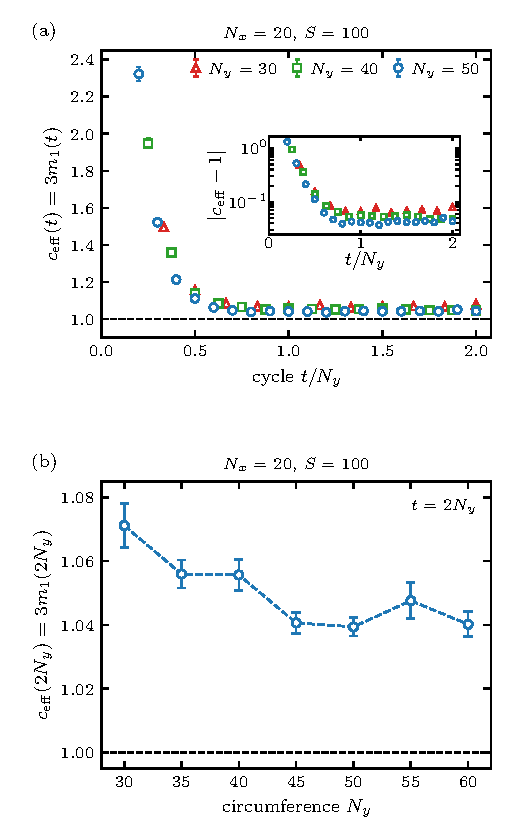
\includegraphics[width=\columnwidth]{Figure_08_central_charge.pdf}
    \caption{\newtext{\textbf{Convergence of the entropy coefficient.} $c_{\rm eff}=3m_1$ is extracted from a free-intercept fit of $\overline S$ versus log chord length over $8\leq A_y\leq N_y/2$. (a) Cycle dependence for $N_y=30,40,50$; the inset resolves $|c_{\rm eff}-1|$. Bars are regression standard errors of the mean-curve slope. (b) Endpoint values after $2N_y$ cycles for $N_y=30,35,\ldots,60$; bars are trajectory SEMs propagated with the covariance between widths. Both panels use $S=100$ independent random-pure trajectories per size and origin averaging, but come from separate ensembles. The horizontal reference is one; connecting lines in (b) are guides.}}
    \label{fig:Ceff}
\end{figure}

{\color{blue}
\section{Purification and the finite-time Lyapunov spectrum}
\label{app:Lyapunov}

The occupation spectrum used in Eq.~\eqref{eq:LyapunovFromOccupations} gives a direct measure of the slow purification modes. Here we explain the relation and its finite-time limitation. The connection between topological Lyapunov boundary modes and slow purification was established in Ref.~\cite{XiaoKawabata2026}; our purpose is to state it in the conventions appropriate to the present circuit.

Equations~\eqref{eq:PurificationKrausProduct} and \eqref{eq:PurificationFermiFunction} relate the maximally mixed initial state to the positive part of its trajectory evolution operator. The same expressions apply to a maximally mixed slab after factoring out an initially pure, decoupled exterior. Projective measurements may make the product singular; logarithms are taken on its nonzero support, with occupations pinned to zero or one assigned infinite single-particle energies. The finite rates and their smallest magnitude are defined in Eq.~\eqref{eq:LyapunovFromOccupations}.

The $\gamma_j(T)$ are finite-time single-particle Lyapunov rates in this normalization. Equivalently, the eigenvalues of $\hat{\mathcal H}_{\rec}$ are obtained from the logarithms of the singular values of $\hat V_{\rec}$, up to a common shift. Its many-body ground state fills the modes with $\gamma_j<0$. When all number sectors on the mixed subsystem are allowed, the lowest excitation changes the occupation of the mode closest to zero and costs $\Delta_{\rec}$. A restriction to one fixed-charge block would instead require a particle--hole excitation; we make no such restriction in this purification experiment.

The entropy in Eq.~\eqref{eq:BinaryEntropy} is a sum of independent mode contributions. Since $h(\nu)=h(1-\nu)$, a nearly pure mode with $T|\gamma_j|\gg1$ contributes
\begin{equation}
    h(\nu_j)=
    \big(1+2T|\gamma_j|\big)e^{-2T|\gamma_j|}
    +O\!\left[(1+T|\gamma_j|)e^{-4T|\gamma_j|}\right].
    \label{eq:PurificationEntropyAsymptotic}
\end{equation}
The modes closest to zero therefore dominate late-time entropy. In real space the same weights multiply their local eigenvector densities in the entropy contour, explaining why the residual entropy follows the wall-localized slow modes. If the finite-time rates converge to a spectrum with a positive smallest magnitude $\Delta$, the entropy has exponential rate $2\Delta$, up to prefactors. A closing gap removes this uniform exponential rate. Neither statement alone fixes the time to reach a prescribed total entropy: the number of contributing modes, finite-time corrections, and record-to-record fluctuations also matter.

The singular-value description for a pure input in Sec.~\ref{sec:Purification} applies along a fixed measurement record. Born probabilities depend on the initial state, so it does not identify the record ensembles generated from pure and maximally mixed inputs.

The plotted $\overline{\Delta}(T)$ is the average of the smallest rate in each record, not the smallest eigenvalue of an averaged generator. Moreover, an exponential rate inferred from typical records need not equal that of the averaged entropy if rare records dominate the latter. We use the gap and its spatial profile as diagnostics of the observed purification, without identifying these distinct averages.

In the size sweep, the observation time grows with circumference as $T=2N_y$. Consequently, finite-time corrections of order $1/T$ can also produce a contribution proportional to $1/N_y$. The observed closing of $\overline{\Delta}(T)$ is consistent with slow boundary dynamics, but extracting an asymptotic dynamical exponent requires convergence in $T$ at fixed $N_y$.
\GPT{Check the gap at longer times at fixed $N_y$ before identifying the fitted size exponent with its asymptotic Lyapunov value.}
}


{\color{blue}
\section{Relaxation gap of the averaged channel}
\label{app:ChannelGap}

Here we relate the two-point relaxation in Eq.~\eqref{eq:CycleChannel} to the many-body channel gap. We consider the perfect occupation resets of Sec.~\ref{sec:Model}, applied in a fixed order that repeats every cycle. The measured modes need not be orthogonal. Let $N$ be the number of single-particle modes, \claudeadd{$P_j=W_jW_j^\dagger$} the projector of the measured OW mode in the convention of Eq.~\eqref{eq:TwoPoint}, and $Q_j=\mathbf{1}-P_j$. The one-cycle map is
\begin{equation}
    \overline G'=A\overline GA^\dagger+B,
    \qquad A=Q_M\cdots Q_1,
    \label{eq:AppCycleChannel}
\end{equation}
where step 1 acts first and $B$ depends only on the target occupations. Thus, deviations from a stationary two-point function obey $\delta G'=A\delta GA^\dagger$. If $a_i$ are the eigenvalues of $A$ and $r=\rho(A)$, the two-point multipliers are $a_i a_j^*$, with largest modulus $r^2$. We assume $r<1$ below.

First, two-point closure gives a bound that does not require Gaussian states. The Heisenberg channel preserves the space spanned by $\hat{\mathbf{1}}$ and the bilinears $\hat c_i^\dagger\hat c_j$. Its spectrum is therefore part of the full channel spectrum. For an invariant sector containing these operators, the largest nonstationary eigenvalue modulus $r_{\rm MB}$ satisfies
\begin{equation}
    r_{\rm MB}\geq r^2,
    \qquad g_{\rm MB}=1-r_{\rm MB}\leq 1-r^2=g_C.
    \label{eq:ChannelGapBound}
\end{equation}
The continuous-time version follows from the inclusion of the covariance generator in the many-body Liouvillian; see Proposition~7 and Eq.~(63) of Ref.~\cite{BarthelZhang2022}. A positive two-point gap alone does not exclude slower higher-order correlations.

For the resets studied here, we can show that the bound is saturated. Choose a single-particle basis beginning with the measured mode $\hat\chi_j$. In this basis, discarding the measurement outcome and applying perfect feedback replaces the measured mode by its target occupation $s_j$. An even operator involving only orthogonal modes is unchanged. An operator with one measured fermion leg is erased, whereas a factor $\hat\chi_j^\dagger\hat\chi_j$ is replaced by $s_j$. The latter reduces the number of fermion operators by two. Consequently, the evolution of a $2p$-point function closes on itself and lower orders. This statement uses the reset action, without Wick factorization.

In the charge-neutral sector, use the normally ordered moments
\begin{equation}
    F^{(p)}_{I;J}=\Tr\!\left(\hat\rho\,
    \hat c_{i_1}^\dagger\cdots\hat c_{i_p}^\dagger
    \hat c_{j_p}\cdots\hat c_{j_1}\right),
    \label{eq:NeutralMomentHierarchy}
\end{equation}
where $I$ and $J$ are increasing $p$-element sets. The highest-order part propagates each creation and annihilation index with $A$ and $A^*$, respectively. Fermionic antisymmetry replaces the single-particle matrices by their exterior powers. The corresponding diagonal block of the moment hierarchy is therefore
\begin{equation}
    \mathcal A_p=(\wedge^p A)\otimes(\wedge^p A)^*.
    \label{eq:ExteriorPowerChannel}
\end{equation}
Here $(\wedge^p A)_{I,J}=\det A[I,J]$; the Cauchy--Binet identity composes the blocks of successive resets in their prescribed order. The lower-order source terms lie off the diagonal and do not change the eigenvalues. The channel multipliers are thus
\begin{equation}
    \Lambda_{I,J}=\prod_{i\in I}a_i\prod_{j\in J}a_j^*,
    \qquad |I|=|J|=p.
    \label{eq:NeutralChannelSpectrum}
\end{equation}
This also holds for nondiagonalizable $A$, as follows by triangularizing it before taking exterior powers. The moments span the neutral operator space: their number is $\sum_{p=0}^N\binom{N}{p}^2=\binom{2N}{N}$.

The constant moment $p=0$ gives the stationary eigenvalue 1. Every other multiplier has modulus at most $r^{2p}\leq r^2$, and the $p=1$ block attains $r^2$ by choosing the same maximal-modulus eigenvalue on both legs. Hence,
\begin{equation}
    g_{q=0}=1-r^2=g_C.
    \label{eq:NeutralChannelGap}
\end{equation}
An even operator with unequal numbers of creation and annihilation operators obeys the same hierarchy, with at least two single-particle factors in each nonconstant block. Its multiplier cannot exceed $r^2$ either. Since the neutral block attains this value, $g_{\rm even}=g_{q=0}$.

Charge neutrality means $[\hat\rho,\hat Q]=0$, with $\hat Q=\sum_i\hat c_i^\dagger\hat c_i$. It permits mixtures of particle-number sectors. Both maximally mixed states and fixed-charge Slater states satisfy this condition, which is preserved by the definite-charge reset Kraus operators even though individual resets can change particle number. Thus Eq.~\eqref{eq:NeutralChannelGap} applies to the states used here. It is not a claim that the circuit preserves a fixed particle-number block.

The dimensionless gap must be distinguished from the decay rate per cycle,
\begin{equation}
    \Delta_{\rm ch}=-\log r_{\rm MB}=-2\log\rho(A),
    \qquad g_C=1-e^{-\Delta_{\rm ch}}.
    \label{eq:ChannelRateVersusGap}
\end{equation}
It is the spectral radius, rather than the largest singular value of $A$, that fixes this asymptotic rate. Jordan blocks and nonnormal evolution can produce polynomial prefactors or transients, so the gap alone does not fix a size-independent mixing time. It also does not determine the purification rate of individual records. The proof concerns exact ordered resets; replacing the cycle by a continuous-time approximation, imperfect feedback, or an average over different schedules requires a separate analysis. The effective continuous-time treatment of Ref.~\cite{BhuiyanPanJian2026} and the general Liouvillian hierarchy of Ref.~\cite{BarthelZhang2022} provide related descriptions, while Eq.~\eqref{eq:NeutralChannelGap} uses the discrete reset structure directly.
}


\bibliographystyle{apsrev4-2}
\bibliography{references}

\end{document}
